
\documentclass[preprint,12pt]{elsarticle}




%% The amsmath package provides various useful equation environments.
\usepackage{amsmath}    % align, cases, etc.
\usepackage{amssymb}    % math symbols
\usepackage{mathtools}  % fixes + extensions to amsmath

%% The amsthm package provides extended theorem environments
\usepackage{amsthm}
\usepackage{hyperref}
\usepackage{adjustbox}
\usepackage{siunitx} %  for better scientific notation
\usepackage{booktabs}
\usepackage{longtable }
\usepackage{graphicx}
\usepackage{subcaption} % for subfigures
\usepackage{algorithm}
\usepackage{algorithmic}

\newtheorem{definition}{Definition}[section]
\newtheorem{theorem}{Theorem}[section]
\newtheorem{lemma}{Lemma}[section]
\newtheorem{assumption}{Assumption}[section]
\usepackage{lineno}

\journal{Reliability Engineering \& System Safety}

\begin{document}
\linenumbers

\begin{frontmatter}


\title{Information Propagation Algorithm for Exact Reliability Analysis in Directed Acyclic Process Networks}

\author[strathclyde]{Temitope Ohiani}\ead{temitope.ohiani@strath.ac.uk}
\author[strathclyde]{Edoardo Patelli\corref{mycorrespondingauthor}} \ead{edoardo.patelli@strath.ac.uk}
\author[nnl]{Caroline Pyke}\ead{caroline.pyke@uknnl.com}

\affiliation[strathclyde]{organization={Department of Civil and Environmental Engineering, University of Strathclyde},
            city={Glasgow},
            country={UK}}

\affiliation[nnl]{organization={United Kingdom National Nuclear Laboratory},
            country={UK}}

  \cortext[mycorrespondingauthor]{Corresponding author}


%% Abstract
\begin{abstract}
Reliability analysis in directed acyclic process networks requires computing, for each node, the probability that at least one viable path exists from any source node to that node. Standard analytical reliability formulations become inaccurate or inefficient in the presence of reconvergent path structures, where multiple paths diverge from shared upstream ancestors and reconverge downstream, thereby creating statistical dependencies that violate path independence assumptions.

This paper presents the Information Propagation Algorithm (IPA), an exact message-passing method that resolves these dependencies through conditional enumeration on shared fork ancestors. IPA processes the network in topological order, applying closed-form updates for independent parent signals and progressive diamond decomposition for dependent reconvergent structures. IPA identifies each diamond subgraph, solves it by conditional probability enumeration, and replaces it with a statistically equivalent supernode. IPA is a specialisation of cutset conditioning, and its cost is computed from the decomposition before the propagation is run.

IPA also propagates interval-valued and probability-box component reliabilities. For interval inputs the propagated range is exact, and for probability-box inputs the bounds on each node's reliability distribution are guaranteed. IPA is validated against an independent binary decision diagram on a benchmark grid network, several real infrastructure networks, and a corpus of 129 random and structured directed acyclic graphs. It reproduces the exact node reliabilities in every case. It is then applied to a medical drone logistics network for Scotland. The analysis identifies the delivery points whose reachability is least certain under the stated input uncertainty. IPA provides exact reliability analysis for a broad class of multi-source directed acyclic process networks, and identifies the structural conditions under which exact inference becomes impractical.
\end{abstract}

%%Research highlights
\begin{highlights}
\item Exact source-to-node reliability for DAGs with reconvergent (diamond) dependence
\item Diamond decomposition with supernode reuse avoids repeated conditioning
\item Per-instance cost follows from the diamond conditioning sets and is known in advance
\item Validated against an exact decision-diagram method on 129 graphs and benchmarks
\item Propagates interval and probability-box component reliabilities natively
\end{highlights}


%% Keywords
\begin{keyword}
Network Reliability \sep Directed Acyclic Graphs \sep Message Passing \sep Reconvergent Structures \sep Imprecise Probability \sep Process Networks \sep Infrastructure Systems
\end{keyword}

\end{frontmatter}

%% Add \usepackage{lineno} before \begin{document} and uncomment 
%% following line to enable line numbers
%% \linenumbers

%% main text
%%


\section{Introduction}

Many infrastructure and engineered systems operate through the propagation of resources and/or information across interconnected components. Examples include electric power networks, water distribution systems, telecommunication networks, transportation systems, and logistics networks. In such systems, functionality depends on the reliability of individual components and on the existence of viable directed paths through which flow can propagate from source nodes to downstream nodes. In this paper, we refer to this class of systems as \emph{multi-source process networks}.
Failures in these systems can have severe operational, economic, environmental, and societal consequences. Their assessment therefore requires metrics that quantify component reliability and the network's ability to preserve connectivity and sustain flow. A natural reliability measure in this context is the probability that at least one viable path exists from one or more source nodes to a given target node. This source-to-node reachability reliability provides a direct measure of the network's ability to maintain function under component and transmission failures.

Directed acyclic graphs (DAGs) are a natural fit to model and evaluate the performance of resource flow systems. In a DAG, nodes represent system components, processing stages, or transfer locations, while directed edges model permissible flow transitions and dependencies between components. Consider the typical process of transport networks where service at downstream locations may depend on the successful operation of several upstream links, hubs, or transfer stages. Failures at earlier stations can cause disruption and delays in travel and, in some cases, stop service altogether.

To mitigate cascading failure scenarios and service bottlenecks, the reliability of the network's resource flow is an important performance metric to monitor. Reliability is generally defined as the probability that a system performs its intended function over a specified time. In flow networks, the intended function is that the other parts of the network successfully receive information flowing from the sources. Complex systems have redundancy strategies and backup paths to ensure this flow. Reliability in multi-source flow networks is the probability that at least one viable operational path exists from source nodes to the other nodes in the network.

The classic approach to exactly solving the reliability problem involves enumerating and combining all possible source-to-node paths. However, this quickly becomes computationally intractable for complex process systems with multiple sources, extensive redundancy, and re-convergent network topologies \cite{george-williams_simulation_2021}. In particular, when distinct paths share upstream nodes or edges before reconverging downstream, the resulting path events are no longer independent, and naïve path-combination rules become invalid.

The structure of DAGs suggests an alternative viewpoint based on message passing. Reliability can be computed locally and recursively by asking, at each node, the probability that at least one viable signal reaches it from any source. For tree-like or conditionally independent substructures, this can be evaluated efficiently using local update rules. However, reconvergent path structures remain problematic because they induce statistical dependencies between incoming signals. These dependencies must be resolved exactly if message passing is to remain accurate.

This paper presents the \emph{Information Propagation Algorithm} (IPA), an exact message-passing method for reliability analysis in directed acyclic process networks. IPA exploits topological ordering to propagate source-to-node reliability from upstream to downstream nodes. Its central idea is to identify reconvergent fork--join subgraphs, referred to here as \emph{diamond structures}, and resolve their dependency explicitly by conditioning on the shared fork ancestors. Once solved, these diamond subgraphs are replaced with statistically equivalent supernodes, and the network is progressively simplified without loss of exactness. An earlier version of the method was presented as the Information Propagation Method~\cite{ohiani_information_2023}. This paper adds a formal complexity analysis, a validation against an independent exact method, and the propagation of imprecise component reliabilities.

The proposed approach preserves exact probability propagation in DAGs with reconvergent structures, where the standard local update introduces an independence error. Decomposing and caching repeated dependency patterns reduces conditional enumeration over already-resolved substructures. The cost on a given network is fixed by the decomposition and known before enumeration begins. The approach also propagates interval-valued and probability-box component reliabilities, so that partial knowledge of the component data is carried through the analysis. These properties suit the method to design-stage studies, where many network configurations are assessed, and to decision problems where the reliability inputs are only partly known.


\subsection{Related Works}\label{subsec:relatedworks}

Early reliability analysis methods are based on relatively simple structural representations of systems. The Reliability Block Diagram (RBD) method~\cite{billinton_network_1992,rausand_m_2014_reliability_2014,ebeling_introduction_2019} models a system as interconnected component blocks arranged in series, parallel, or $k$-out-of-$n$ configurations, whose reliability can be computed using closed-form expressions. While computationally efficient and intuitive, RBDs are limited in their ability to represent complex dependency structures and reconvergent flows. Extensions such as Dynamic Reliability Block Diagrams (DRBD)~\cite{distefano_dynamic_2007} incorporate time-dependent behaviour and allow more realistic modelling of component interactions and system dependencies, but they still struggle to represent highly interconnected networks with multiple convergent paths.

Boolean logic-based methods provide a more flexible framework for modelling system failure mechanisms by including event causes and consequences. Fault Tree Analysis (FTA) \cite{xing_fault_2008} is a top-down deductive logic tree to identify possible combinations of component failures that could cause specific undesirable events. Event Tree Analysis (ETA) is the complementary inductive method where the logic tree instead begins with the initiating event and traces all possible sequences of subsequent successes and failures through branching structures and logic gates \cite{cepin_event_2011}.  These methods can capture a wider range of logical dependencies than RBDs; however, for large-scale systems they require extensive manual construction and become difficult to maintain. In addition, their computational cost grows rapidly with the size and complexity of the logical expressions, particularly in systems with multiple interacting pathways~\cite{sherwin_fault_1993,xing_fault_2008}.

The main limitations of tree-based methods stem from exponential growth in logic expressions and manual construction requirements for complex systems. Binary Decision Diagrams (BDDs)\cite{rauzy_new_1993,bryant_graph-based_1986, brace_efficient_1990} were adapted from circuit design to improve fault tree models by using variable elimination and path reduction techniques on Boolean functions. In BDDs, Boolean functions are represented as directed acyclic graphs (DAGs) based on Shannon decomposition, where each non-sink node represents a Boolean variable with two outgoing edges corresponding to the variable being true or false \cite{xing_fault_2008}. This structure allows BDD-based methods to require less memory and computational time than traditional fault tree analysis \cite{rauzy_new_1993}.
BDD algorithms can handle complex Boolean expressions with thousands of variables while maintaining polynomial space complexity for many systems. However, their performance depends critically on variable ordering, and determining an optimal ordering is computationally intractable in general~\cite{bryant_ordered_nodate}. For highly interconnected networks with shared components and reconvergent fan-out, BDD construction meets the reconvergence problem. Multiple paths converging at common nodes require extensive intermediate node generation, which can exceed memory limitations even for moderately sized systems. These challenges become severe when modelling common cause failures and dependency structures that propagate through many interconnected pathways.

Common cause failures create statistical dependencies that violate the independence assumptions underlying traditional reliability calculations\cite{mosleh_estimation_nodate}. When multiple components share common failure modes, the resulting dependency patterns cannot be captured efficiently through simple Boolean combinations. This is a limitation shared by RBDs, FTAs, and BDDs in process systems with convergent network topologies.

To overcome these limitations, path-based and graph-theoretic methods have been developed. These methods treat the network as a probabilistic graph problem and apply probability mathematics and set operations to compute network reliability. Exact methods based on minimal path sets and minimal cut sets~\cite{kumar_composite_2018,li_cuttie_2005,billinton_network_1992,liu_improved_2012} identify the smallest collections of components that maintain connectivity or cause system failure. Recursive decomposition techniques improve efficiency by partitioning the network into smaller subproblems. For example, the cut-based method in~\cite{liu_improved_2012} uses both the disjoint minimal cut sets and the disjoint minimal path sets during decomposition for networks with low edge reliabilities. Kim and Kang's method \cite{kim_network_2013} extends the Recursive Decomposition Algorithm through a Logical Expansion approach (LE-RDA) that uses separate intersection and union operations to decompose general system events with multiple node pairs. Nevertheless, these methods remain computationally expensive for networks with extensive redundancy and reconvergent connectivity, as they still require combinatorial enumeration of path or cut structures.

Simulation methods such as Monte Carlo (MC) have become a widely adopted reliability analysis method for complex networks \cite{fishman_comparison_1986}. MC algorithms can handle arbitrary network structures and provide confidence intervals, although they can become computationally expensive for large networks requiring many samples to reach acceptable accuracy. Monte Carlo variants such as importance sampling\cite{hui_monte_2007} and subset simulation \cite{au_estimation_2001} have been proposed to address rare failure events, though these optimisations often demand more computational cost.

More recently, message passing approaches based on probabilistic graphical models have been explored for network reliability analysis~\cite{yedidia_understanding_2003,pearl_probabilistic_1988}. These methods infer system reliability by exploiting the network structure to propagate local calculations until convergence. Message passing scales linearly with network size and handles complex dependency structures directly. For instance, the directed Probability Propagation Method (dPrPm)~\cite{tong_probability_2019} handles dependencies through pairwise probability tracking and approximation of joint distributions. While effective, these approaches can become memory-intensive and computationally demanding as the number of dependent interactions increases. In addition, convergence is not always guaranteed~\cite{murphy_loopy_2013}, and approximation quality depends heavily on network topology and component correlation strength.

Exact inference in probabilistic graphical models resolves a dependency induced by shared ancestry either by conditioning or by clustering. Cutset conditioning enumerates the states of a set of variables whose removal leaves the rest of the structure singly connected~\cite{pearl_probabilistic_1988}. The junction-tree algorithm groups variables into a tree of clusters, and its cost is exponential in the treewidth of the network~\cite{lauritzen_local_1988}. Both are exact, and both are governed by a structural width of the graph. IPA specialises cutset conditioning to the source-to-node reachability problem, and its cost is governed by the same width parameter as junction-tree inference and a well-ordered binary decision diagram (Section~\ref{sec:complexity}).

A component failure probability is often known only within bounds, from sparse operational data or expert judgement. Such a value is represented as an interval, asserting only that the true reliability lies between two bounds, or as a probability box, a pair of bounding cumulative distribution functions~\cite{ferson_constructing_2003}. Williamson and Downs~\cite{williamson_probabilistic_1990} give the arithmetic on probability boxes under known or unknown dependence, on the classical Fr\'echet--Hoeffding bounds for joint distributions. A binary decision diagram can be extended to interval-valued inputs, using the same monotonicity IPA relies on~\cite{jacob_uncertainty_2011}. The construction does not scale. Its result also depends on the variable ordering, so a conservative envelope over several orderings is needed~\cite{imakhlaf_extending_2017}. IPA propagates interval and probability-box reliabilities through the same conditioning it applies to point values, without an ordering or a separate monotonicity check.

Hence, existing methods face a trade-off between generality, computational efficiency, and exactness. Classical analytical methods struggle with complex dependency structures, exact path-based approaches suffer from combinatorial explosion, and simulation or approximate message-passing methods sacrifice exactness for scalability. This work addresses this gap by proposing an exact message-passing framework for DAG reliability analysis that explicitly resolves reconvergent dependencies through conditional decomposition of fork--join substructures. By identifying and reducing these structures during computation, the proposed method avoids repeated enumeration over shared dependencies and preserves exact probabilistic results.

\section{Network Model}\label{sec:model}
A process system is modelled as a directed acyclic graph $G = (V, E)$ where $V$ denotes the set of nodes (components) and $E \subseteq V \times V$ represents the set of directed edges (dependencies). Let $S \subseteq V$ denote the set of source nodes and $T \subseteq V$ the set of sink nodes. Throughout the paper we use $\text{Pa}(v)$ and $\text{Ch}(v)$ to represent the set of parent nodes and child nodes of $v$, respectively.

\subsection{Component States and Probabilistic Model}

Each node $v \in V$ is associated with a binary random variable $X_v \in \{0,1\}$, where $X_v = 1$ indicates that node $v$ is operational. Similarly, each directed edge $(u,v) \in E$ is associated with a binary random variable $X_{uv} \in \{0,1\}$ representing successful transmission from $u$ to $v$.

We define:
\begin{itemize}
\item $R(v) = P(X_v = 1)$: intrinsic reliability of node $v$
\item $P(u,v) = P(X_{uv} = 1)$: transmission probability of edge $(u,v)$
\end{itemize}

A directed path $\pi(s,v) = (s = v_0, v_1, \ldots, v_k = v)$ is said to be \emph{viable} if all nodes and edges along the path are operational, i.e.
\[
X_{v_0} X_{v_1} \cdots X_{v_k} \cdot X_{v_0 v_1} \cdots X_{v_{k-1} v_k} = 1.
\]

\begin{definition}[Viable Path]
A path $\pi(s,v)$ from source $s \in S$ to node $v \in V$ is viable if all nodes and edges along the path are functional.
\end{definition}

\begin{figure}[htbp]
  \centering
  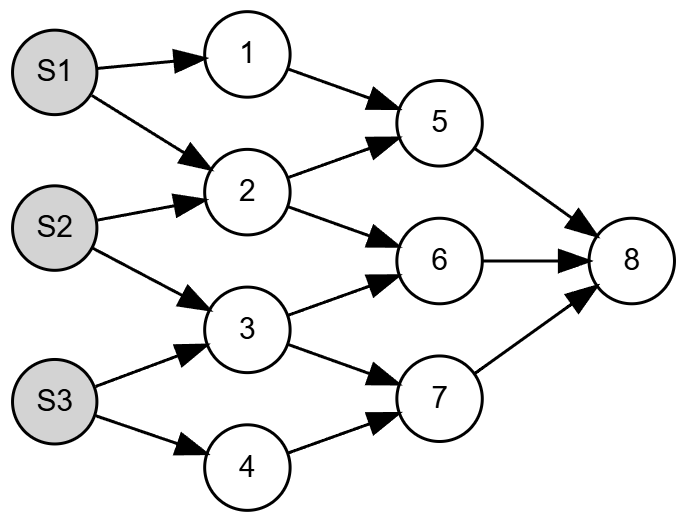
\includegraphics[scale=0.3]{images/simpleDag.png}
  \caption{A Multi-Source Directed Acyclic Graph.}
  \label{fig:dag_rbd}
\end{figure}

\subsection{Definition of Diamond Structures}

We formalise reconvergent dependency patterns through the notion of a diamond subgraph.

\begin{definition}[Diamond Structure]
A diamond structure is a subgraph $D \subseteq G$ characterised by:
\begin{itemize}
    \item a set of fork nodes $F \subseteq V$, where each $f \in F$ has at least two outgoing paths,
    \item a join node $j \in V$ with at least two incoming paths,
    \item at least two distinct directed paths from nodes in $F$ to $j$,
    \item at least one shared upstream node or edge among these paths.
\end{itemize}
\end{definition}

In such structures, the paths from fork nodes to the join node are not independent because they share common components. The simplest case is a \emph{single-fork diamond}, where all reconvergent paths originate from a single fork node.

\subsection{Reliability Objective}

The reliability problem is formally stated as computing the probability that there is at least one viable path from any source node to each target node in the network. The reachability probability of a node $v \in V$ is defined as the probability that at least one viable path exists from any source node to $v$:
\begin{equation}
b(v) = P\left( \bigcup_{s \in S} \bigcup_{\pi \in \Pi(s,v)} 
\{\pi \text{ is viable}\} \right),
\end{equation}
where $\Pi(s,v)$ denotes the set of all directed paths from $s$ to $v$.

The quantity $b(v)$ represents the probability that node $v$ receives flow from at least one source and is referred to as the \emph{node reliability} (or belief) at $v$.

The reachability of $v$ can also be written recursively. With $X_v$ and $X_{uv}$ the node and edge indicators,
\begin{equation}\label{eq:reach_indicator}
\mathcal{R}_v = X_v \wedge \Bigl( v \in S \;\vee\; \bigvee_{u \in \text{Pa}(v)} \bigl( \mathcal{R}_u \wedge X_{uv} \bigr) \Bigr),
\end{equation}
and $b(v) = P(\mathcal{R}_v = 1)$. Because the component indicators are mutually independent (Assumption~\ref{as:indep}), $\mathcal{R}_v$ is a monotone Boolean function of them: restoring a failed component can create source-to-node connectivity but never remove it. Computing $b(v)$ is \#P-hard in general, since two-terminal network reliability is a special case~\cite{valiant_complexity_1979,ball_complexity_1980}. The monotonicity makes $b(v)$ non-decreasing in every node prior and every edge probability, which Section~\ref{subsec:impreciseinputs} uses to propagate interval-valued inputs exactly.

For a node $v$, let $\text{anc}(v)$ be its ancestors, the nodes with a directed path to $v$. Given a set $C$ of forks whose reachability states are fixed by conditioning, the \emph{unresolved influence} of a parent $u$ of a join is
\begin{equation}\label{eq:infl}
\text{infl}(u; C) = \bigl( \{u\} \cup \text{anc}(u) \bigr) \setminus C ,
\end{equation}
the upstream components on which the signal through $u$ still depends. Two parents of a join are statistically dependent when their unresolved influences intersect. This is the structural test used by the decomposition of Section~\ref{sec:decomp}.


\subsection{Model Assumptions}

\begin{assumption}[Graph Structure]
The network $G$ is a directed acyclic graph (i.e. $G$ contains no directed cycles), and every node $v \notin S$ is reachable from at least one source node.
\end{assumption}

\begin{assumption}[Component Independence]\label{as:indep}
Node states $\{X_v\}$ and edge states $\{X_{uv}\}$ are mutually independent. Node and edge states are also independent of each other.
\end{assumption}

\begin{assumption}[Binary Operation]
All nodes and edges have binary states (operational or failed).
\end{assumption}

Dependencies between paths arise solely from shared nodes or edges. In particular, signals arriving at a node from different parents are independent only if the corresponding upstream paths do not share common components. This formulation is equivalent to a network reliability problem with node and edge failures, where the objective is to compute source-to-node reachability probabilities.

\subsection{Imprecise Component Reliabilities}\label{subsec:impreciseinputs}

The model above takes the component reliabilities $R(v)$ and $P(u,v)$ as known point values. In many applications these inputs are themselves uncertain: a failure probability may be estimated from sparse operational data or elicited from an expert. Each component reliability is therefore allowed in one of three forms of increasing informativeness:
\begin{enumerate}
    \item a point value $p \in [0,1]$, as above;
    \item an interval $[\underline{p}, \overline{p}] \subseteq [0,1]$, asserting only that the true reliability lies between the stated bounds;
    \item a probability box: a pair of cumulative distribution functions $(\underline{F}, \overline{F})$ that bound the distribution of the uncertain reliability, appropriate when partial distributional information is available~\cite{ferson_constructing_2003,williamson_probabilistic_1990}.
\end{enumerate}
The reliability objective generalises with the input. For an interval input, the target is the exact range $[\underline{b}(v), \overline{b}(v)]$ of node reliabilities over all component reliabilities consistent with the stated intervals. For a probability-box input, the target is a sound pair of bounds on the distribution of $b(v)$. Section~\ref{sec:imprecise} shows that the propagation scheme computes the interval range exactly, by the monotonicity established above, and computes guaranteed distributional bounds in the probability-box case.

\section{The Information Propagation Algorithm}\label{sec:IPA}

The Information Propagation Algorithm (IPA) computes source-to-node reliability in a directed acyclic graph by propagating reachability probabilities from upstream nodes to downstream nodes in topological order. For each node $v \in V$, the objective is to compute
\begin{equation}
b(v) = P(\text{at least one viable path from any source to } v),
\end{equation}
where $b(v)$ denotes the reliability of node $v$.

\subsection{Signal Propagation Formulation}

Let $v$ be a non-source node with parent set
\[
\text{Pa}(v) = \{p_1, p_2, \ldots, p_k\}.
\]
For each parent $p_i \in \text{Pa}(v)$, define the incoming signal event
\[
A_i = \{\text{a viable signal reaches } v \text{ through parent } p_i\}.
\]
The corresponding signal probability is
\begin{equation}
S_i = P(A_i) = b(p_i)\,P(p_i,v),
\end{equation}
that is, the probability that a viable path reaches $p_i$ and is successfully transmitted through edge $(p_i,v)$.

Since node $v$ must itself be operational in order to receive and transmit flow, its reliability is
\begin{equation}
b(v) = R(v)\,P\left(\bigcup_{i=1}^{k} A_i\right).
\label{eq:general_belief_update}
\end{equation}

For a source node $v_s \in S$, reliability is simply its intrinsic reliability:
\begin{equation}
b(v_s) = R(v_s).
\label{eq:source_update}
\end{equation}

\subsection{Topological Evaluation Strategy}

Because the network is acyclic, node reliabilities can be evaluated in topological order. Let
\[
L = \{L_1, L_2, \ldots, L_K\}
\]
denote a layering of the graph such that every edge goes from an earlier layer to a later one. Then, for any node $v \in L_i$, all parent nodes $p \in \text{Pa}(v)$ belong to layers $L_j$ with $j < i$.

This property allows IPA to evaluate all node reliabilities in a single forward pass:
\begin{itemize}
    \item source nodes are initialised using \eqref{eq:source_update};
    \item each non-source node is processed once all parent reliabilities are available;
    \item the local update depends on whether the incoming parent signals are independent or dependent.
\end{itemize}

No iterative convergence procedure is required.

\subsubsection{Independent Parent Signals}

If the incoming signal events $\{A_i\}_{i=1}^{k}$ are mutually independent, then the probability that node $v$ receives at least one signal is
\begin{equation}
P\left(\bigcup_{i=1}^{k} A_i\right)
= 1 - \prod_{i=1}^{k}(1-S_i).
\label{eq:independent_union}
\end{equation}
Substituting \eqref{eq:independent_union} into \eqref{eq:general_belief_update} gives
\begin{equation}
b(v) = R(v)\left[1-\prod_{p \in \text{Pa}(v)}\left(1-b(p)P(p,v)\right)\right].
\label{eq:independent_update}
\end{equation}

Equation \eqref{eq:independent_update} is exact when the upstream paths associated with the incoming parent signals do not share common nodes or edges. Two important special cases are shown in Figures~\ref{fig:chain} and~\ref{fig:indepmulti}.

For a node with a single parent $p$, the update reduces to the chained-path case
\begin{equation}
b(v) = R(v)\,b(p)\,P(p,v).
\label{eq:single_parent_update}
\end{equation}

\begin{figure}[htbp]
  \centering
  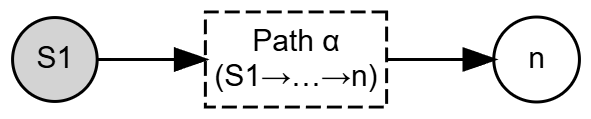
\includegraphics[scale=0.35]{images/chain.png}
  \caption{Single-path structure: chained signal propagation.}
  \label{fig:chain}
\end{figure}

\begin{figure}[htbp]
  \centering
  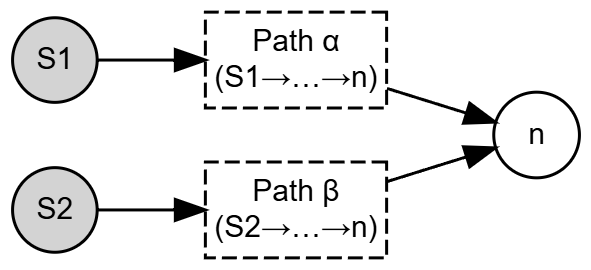
\includegraphics[scale=0.35]{images/indepmulti.png}
  \caption{Multiple independent parent signals: parallel signal propagation.}
  \label{fig:indepmulti}
\end{figure}

\subsubsection{Reconvergent Structures and Independence Breakdown}

The update rule in \eqref{eq:independent_update} is no longer exact when the incoming signal events are dependent. In directed acyclic graphs, this occurs in \emph{reconvergent structures}, where multiple upstream paths share common components before merging at a downstream node.

Let $v$ be a join node receiving signals from parents $\{p_1,p_2\}$. If the upstream paths leading to $p_1$ and $p_2$ share a common ancestor $f$, then the events $A_1$ and $A_2$ are dependent. In that case, applying the independence-based rule
\begin{equation}
P(A_1 \cup A_2) = 1-(1-S_1)(1-S_2)
\label{eq:wrong_indep_formula}
\end{equation}
overestimates the true probability of signal reception, because it ignores the correlation induced by the shared upstream components.

IPA resolves this problem by identifying such reconvergent structures and conditioning on the shared upstream variables that induce the dependency.

\subsubsection{Diamond Structures and Conditional Decomposition}

The fundamental dependency-inducing pattern considered by IPA is a \emph{diamond structure}: a reconvergent fork--join subgraph in which multiple paths diverge from one or more shared upstream nodes and reconverge at a join node.

Consider a single-fork diamond with fork node $f$ and join node $j$. Let
\[
J = \{\text{a signal reaches } j\}, \qquad
F = \{\text{fork node } f \text{ is operational}\}.
\]
By the law of total probability,
\begin{equation}
P(J) = P(J \mid F)P(F) + P(J \mid \bar{F})P(\bar{F}).
\label{eq:diamond_ltp}
\end{equation}

Conditioning on the state of the fork restores independence among the downstream paths:
\begin{itemize}
    \item if $F=1$, the fork is active and the paths downstream of $f$ become conditionally independent;
    \item if $F=0$, no signal can propagate through paths originating from $f$.
\end{itemize}

Thus, if the diamond contains $k$ downstream paths from $f$ to $j$, then
\begin{equation}
P(J \mid F) = 1-\prod_{i=1}^{k}\left(1-S_i^{(F)}\right),
\label{eq:diamond_conditional_update}
\end{equation}
where $S_i^{(F)}$ denotes the probability that path $i$ transmits a signal to $j$ given that the fork is active.

For a simple induced diamond with no alternative upstream routes to the join node,
\begin{equation}
P(J \mid \bar{F}) = 0.
\label{eq:diamond_no_alternative}
\end{equation}

\subsubsection{Generalisation to Multiple Conditioning Nodes}

More complex reconvergent structures may involve several shared upstream nodes
\[
\mathcal{C} = \{c_1,c_2,\ldots,c_m\}.
\]
In that case, the join-node signal probability is computed by enumerating all conditioning states:
\begin{equation}
P(J) = \sum_{s \in \{0,1\}^{m}} P(J \mid s)\,P(s),
\label{eq:multi_conditioning}
\end{equation}
where $s=(s_1,\ldots,s_m)$ is a binary assignment to the conditioning nodes and
\begin{equation}
P(s)=\prod_{i=1}^{m}[b(c_i)]^{s_i}[1-b(c_i)]^{1-s_i}.
\label{eq:state_probability}
\end{equation}

For each conditioning state $s$, the remaining incoming paths to the join node become conditionally independent, so the local update can again be evaluated using the independent-signal formula.

\subsection{Simple Example}\label{sec:simple_example}

To illustrate the effect of reconvergent dependencies and the correctness of the conditioning approach, consider the simple diamond in Figure~\ref{fig:numerical-diamond}. The subgraph consists of a single fork--join pair connected by two intermediate paths. All non-source nodes have intrinsic reliability $0.9$, and all edges have transmission probability $0.9$.

\begin{figure}[htbp]
\centering
  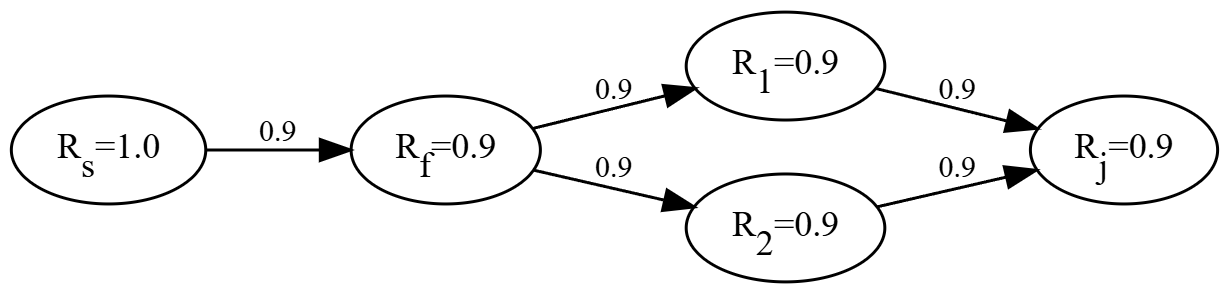
\includegraphics[scale=0.3]{images/numerical-diamond.png}
\caption{A simple diamond subgraph between fork node $f$ and join node $j$.}
\label{fig:numerical-diamond}
\end{figure}

\subsubsection{Solution by Path Enumeration (Correct but Expensive)}

We enumerate the relevant fork/intermediate-node states:
\begin{align*}
P_1 &= 0.81 \times 0.81 \times 0.81 = 0.531441 
    && \text{(fork active, both intermediates work)}, \\
P_2 &= 0.81 \times 0.81 \times 0.19 = 0.124659
    && \text{(fork active, only first intermediate works)}, \\
P_3 &= 0.81 \times 0.19 \times 0.81 = 0.124659
    && \text{(fork active, only second intermediate works)}, \\
P_4 &= 0.81 \times 0.19 \times 0.19 = 0.029241
    && \text{(fork active, both intermediates fail)}, \\
P_5 &= 0.19
    && \text{(fork inactive, no signal possible)}.
\end{align*}

The signal-reception probabilities at the join node are
\[
P(\text{signal}) =
\begin{cases}
0.99, & \text{if both paths send signals}, \\
0.9,  & \text{if only one path sends a signal}, \\
0,    & \text{if no path sends a signal}.
\end{cases}
\]

Hence,
\begin{align*}
P(\text{signal})
&= P_1 \times 0.99 + P_2 \times 0.9 + P_3 \times 0.9 \\
&= 0.531441 \times 0.99 + 0.124659 \times 0.9 + 0.124659 \times 0.9 \\
&= 0.75051279.
\end{align*}
The resulting reliability at the join node is
\[
b(j)=R(j)\,P(\text{signal})=0.9 \times 0.75051279 = 0.675461511.
\]

\subsubsection{Solution by Independent Update (Incorrect)}

Using the independent-parent update yields
\begin{align*}
b(f) &= R(s)\,P(s,f)\,R(f) = 1.0 \times 0.9 \times 0.9 = 0.81, \\
b(p_1)=b(p_2) &= b(f)\,P(f,p)\,R(p) = 0.81 \times 0.9 \times 0.9 = 0.6561.
\end{align*}
Thus,
\[
S_1 = S_2 = b(p_i)\,P(p_i,j) = 0.6561 \times 0.9 = 0.59049.
\]
Treating the two incoming signals as independent gives
\begin{align*}
P(\text{signal}) &= 1-(1-0.59049)^2 = 0.83230, \\
b(j) &= 0.9 \times 0.83230 = 0.749071,
\end{align*}
which overestimates the correct value.

\subsubsection{Solution by Diamond Conditioning (Correct and Efficient)}

Conditioning on the fork state, we have
\[
b(f)=0.81.
\]
If the fork is active, each downstream path has conditional transmission probability
\[
P(f,p)\,R(p)\,P(p,j)=0.9 \times 0.9 \times 0.9 = 0.729.
\]
Therefore,
\begin{align*}
P(\text{signal}\mid F=1) &= 1-(1-0.729)^2 = 0.926559, \\
P(\text{signal}\mid F=0) &= 0.
\end{align*}
Using \eqref{eq:diamond_ltp},
\begin{align*}
P(\text{signal})
&= P(\text{signal}\mid F=1)P(F=1) + P(\text{signal}\mid F=0)P(F=0) \\
&= 0.926559 \times 0.81 + 0 \times 0.19 \\
&= 0.75051279.
\end{align*}
Hence,
\[
b(j)=0.9 \times 0.75051279 = 0.675461511,
\]
which matches the exact path-enumeration result.

This example shows the central idea behind IPA: the dependence induced by a reconvergent structure can be handled exactly by conditioning only on the shared upstream variables that generate the dependence.

\subsection{IPA Workflow and Algorithm}

The Information Propagation Algorithm computes node reliability in a single forward pass over the DAG. For each node, the algorithm:
\begin{itemize}
    \item computes incoming signal probabilities from its parent nodes;
    \item applies the closed-form independent update when the parent signals are independent;
    \item detects reconvergent structures when dependencies are present;
    \item resolves those dependencies through conditional enumeration on shared upstream nodes.
\end{itemize}

This formulation localises exact dependency handling to the subgraphs that require it. Elsewhere, it retains the simple closed-form updates.

Algorithm~\ref{alg:ipa} summarises the overall computation.

\begin{algorithm}[h]
\caption{Information Propagation Algorithm (IPA)}
\label{alg:ipa}
\begin{algorithmic}[1]
\STATE Compute a topological ordering of $G$
\FOR{each node $v \in V$ in topological order}
    \IF{$v \in S$}
        \STATE $b(v) \gets R(v)$
    \ELSE
        \STATE Compute $S_i = b(p_i)\,P(p_i,v)$ for all $p_i \in \text{Pa}(v)$
        \IF{incoming parent signals are independent}
            \STATE $b(v) \gets R(v)\left[1-\prod_i (1-S_i)\right]$
        \ELSE
            \STATE Identify reconvergent (diamond) structures affecting $v$
            \STATE Resolve dependencies by conditional enumeration
            \STATE Compute $b(v)$ from the conditioned signal probabilities
        \ENDIF
    \ENDIF
\ENDFOR
\RETURN $\{b(v)\}_{v \in V}$
\end{algorithmic}
\end{algorithm}

\subsubsection{Computational Characteristics}

For nodes with independent parent signals, the update cost is $O(|\text{Pa}(v)|)$, so the total computational cost is linear in the number of edges for tree-structured networks.

For nodes involved in reconvergent structures, additional cost arises from conditional enumeration over shared upstream components. If a diamond requires conditioning on $c$ shared upstream variables, the local cost scales as $O(2^c)$, independent of the total number of full path combinations. The practical efficiency of IPA therefore depends primarily on the number and nesting depth of such dependency-inducing structures.

The next section introduces a progressive decomposition strategy that reduces repeated conditioning by replacing resolved diamond subgraphs with statistically equivalent supernodes.


\section{Progressive Decomposition of Diamond Structures}\label{sec:decomp}
Progressive decomposition aims to make IPA practical on non-trivial DAGs with reconvergent structure. By replacing resolved diamonds with conditionally equivalent supernodes, it preserves exactness and improves efficiency: the same dependencies are never conditioned on repeatedly.

Real process networks rarely contain only isolated diamonds. Reconvergent structures often overlap or nest within one another, so that the output of one diamond becomes part of a larger downstream reconvergent structure. Repeatedly conditioning on the same upstream variables here causes computational redundancy: for a network with $L$ nested dependency levels, a direct conditional evaluation may require
\begin{align}
b(j) = & R(j) \cdot
\sum_{s_1 \in \{0,1\}^{m_1}}
\sum_{s_2 \in \{0,1\}^{m_2}}
\cdots \nonumber \\
&
\sum_{s_L \in \{0,1\}^{m_L}}
P(s_1)P(s_2\mid s_1)\cdots P(s_L\mid s_1,\ldots,s_{L-1})
\,\phi(s_1,\ldots,s_L),
\label{eq:nested_direct_enum}
\end{align}
where $m_\ell$ is the number of conditioning nodes introduced at nesting level $\ell$, and $\phi(\cdot)$ is the resulting signal probability at the join node. The cost of this direct evaluation grows exponentially with both the number of conditioning variables and the depth of nesting. Progressive decomposition avoids the repeated re-evaluation behind \eqref{eq:nested_direct_enum} by solving each diamond once, storing its exact conditional behaviour in a \emph{supernode}, and reusing that behaviour whenever the reduced network is evaluated further downstream.

\subsection{Supernode Representation and Exactness Guarantees}\label{sec:supernode}

Let $D$ be a diamond subgraph with fork-side conditioning set
\[
\mathcal{C}_D = \{c_1,\ldots,c_m\}
\]
and join node $j_D$. Solving the diamond yields the exact conditional signal probability at the join node for every configuration of the conditioning variables:
\begin{equation}
\psi_D(s) = P(J_D \mid s),
\qquad s \in \{0,1\}^{m},
\label{eq:supernode_conditional_map}
\end{equation}
where $J_D$ denotes the event that a signal reaches the join node of the diamond and $s$ is a binary state assignment to $\mathcal{C}_D$. The resolved diamond is then replaced by a supernode that stores the map $s \mapsto \psi_D(s)$: whenever the conditioning state $s$ is encountered in a larger downstream computation, the contribution of the original diamond is recovered exactly through \eqref{eq:supernode_conditional_map}, without re-solving the full subgraph. The following four results make this exact, in order: that a resolved diamond's conditional map does not depend on the outer context it sits in; that conditioning on a shared fork is what makes the map well defined; that independent reconvergent structures at the same join can each be resolved on its own separating set, without joint conditioning over the combined ancestry; and that the supernode replacement is therefore lossless downstream.

\begin{lemma}[Conditional Invariance]\label{lem:invariance}
Let $D$ be a diamond subgraph with join $j_D$ and conditioning set $C \subseteq \mathcal{C}_D$, and let $\psi_D(s) = P(\mathcal{R}_{j_D}=1 \mid \mathcal{R}_C = s)$, $s \in \{0,1\}^{|C|}$, be its conditional signal map. If an enclosing computation conditions on further variables $A$ disjoint from the nodes and edges internal to $D$, then $\psi_D(s)$ is unchanged by that outer conditioning.
\end{lemma}

\begin{proof}
Fix $s$. Conditional on $\mathcal{R}_C=s$, the event $\{\mathcal{R}_{j_D}=1\}$ is a deterministic function, by \eqref{eq:reach_indicator}, of the node and edge indicators internal to $D$. By Assumption~\ref{as:indep} these indicators are independent of every indicator outside $D$, in particular of the variables in $A$. Hence $P(\mathcal{R}_{j_D}=1\mid \mathcal{R}_C=s,\mathcal{R}_A=a)=\psi_D(s)$ for every outer state $a$: the outer conditioning changes only the probability with which a state $s$ occurs, never the value $\psi_D(s)$ itself.
\end{proof}

The disjointness required by Lemma~\ref{lem:invariance} is what identification enforces (Section~\ref{sec:identification}): whenever an outer state does fix a variable internal to a previously resolved diamond, the sub-problem it defines is a different one and is resolved, and stored, separately.

\begin{lemma}[Separator Sufficiency]\label{lem:separator}
Let $v$ be a join node and let $C \subseteq F \cap \mathrm{anc}(v)$ be a set of forks such that $\mathrm{infl}(u;C)\cap\mathrm{infl}(u';C)=\emptyset$ for every pair of distinct parents $u,u'\in\mathrm{Pa}(v)$, where $\mathrm{infl}$ is defined in \eqref{eq:infl}. Then, conditional on $\mathcal{R}_C$, the parent reachability events $\{\mathcal{R}_u\}_{u\in\mathrm{Pa}(v)}$ are mutually independent, and
\begin{equation}
b(v\mid \mathcal{R}_C=s) = R(v)\left(1-\prod_{u\in\mathrm{Pa}(v)}\bigl(1-P(\mathcal{R}_u=1\mid \mathcal{R}_C=s)\,P(u,v)\bigr)\right).
\end{equation}
\end{lemma}

\begin{proof}
With $\mathcal{R}_C$ fixed, each $\mathcal{R}_u$ is, by \eqref{eq:reach_indicator}, a function of the indicators in $\mathrm{infl}(u;C)$ alone. These sets are disjoint across parents by hypothesis, and functions of disjoint sets of mutually independent indicators (Assumption~\ref{as:indep}) are themselves independent. The stated update is then \eqref{eq:independent_update} applied conditionally on $\mathcal{R}_C=s$.
\end{proof}

Lemma~\ref{lem:separator} is what the unresolved-influence test of \eqref{eq:infl} is for: identification returns, for each reconvergent structure, a conditioning set with this separating property, so the resulting cost is $2^{|C|}$.

\begin{lemma}[Independent-Substructure Factorisation]\label{lem:factorisation}
Fix a conditioning context $E$ and write $u\sim u'$ for parents $u,u'$ of a join $v$ whenever $\mathrm{infl}(u;E)\cap\mathrm{infl}(u';E)\neq\emptyset$. Let $G_1,\ldots,G_m$ be the equivalence classes of $\mathrm{Pa}(v)$ under the transitive closure of $\sim$. The events $\{v\text{ is reached through some parent in }G_k\}$, $k=1,\ldots,m$, are mutually independent, and
\begin{equation}
b(v) = R(v)\left(1-\prod_{k=1}^{m}\bigl(1-P(v\text{ reached via }G_k)\bigr)\right),
\end{equation}
so each group $G_k$ can be resolved on its own separating set $C_k$ (Lemma~\ref{lem:separator}) independently of the others.
\end{lemma}

\begin{proof}
Distinct classes have disjoint unresolved influence by construction, so the class events are functions of disjoint sets of mutually independent indicators, hence independent by Assumption~\ref{as:indep}; the product form is \eqref{eq:independent_update} applied to the $m$ group events.
\end{proof}

At a join whose parents form $m$ independent groups with conditioning sets $C_1,\ldots,C_m$, joint conditioning over the combined shared ancestry would enumerate $2^{|C_1|+\cdots+|C_m|}$ states. Lemma~\ref{lem:factorisation} enumerates $\sum_{k=1}^m 2^{|C_k|}$ states instead. For $k$ parents each depending on its own independent fork, this reduces the cost from $2^k$ to $2k$, from exponential to linear in the fan-in.

\begin{lemma}[Supernode Equivalence]\label{lem:supernode}
Let $D$ be a resolved diamond, or a resolved independent group $G_k$ of Lemma~\ref{lem:factorisation}, with conditional signal map $\psi_D(s)$. Replacing $D$ by a supernode storing $\psi_D(s)$ preserves the exact source-to-node reliability of every downstream node in the reduced graph.
\end{lemma}

\begin{proof}
The contribution of $D$ to any downstream computation enters only through the probability that its join receives a signal under a given conditioning state. By Lemma~\ref{lem:invariance} the stored map equals $\psi_D(s)$ in every outer context that fixes no variable internal to $D$, and by Lemmas~\ref{lem:separator} and~\ref{lem:factorisation} the downstream update combines this map with the remaining parent signals through the same independent-union rule used elsewhere in IPA. Both are preserved by the replacement, so every downstream belief is unchanged.
\end{proof}

\subsection{Progressive Decomposition Procedure}\label{sec:procedure}

IPA applies diamond decomposition progressively as it processes the network in topological order. When it reaches a join node whose parent signals are dependent, it partitions the parents into independent groups by testing pairwise intersection of their unresolved influence, \eqref{eq:infl} (Lemma~\ref{lem:factorisation}). For each group it finds the earliest fork common to its members and the subgraph this induces, computes the group's conditional signal map by conditioning on that fork (Lemma~\ref{lem:separator}), and replaces the resolved group by a supernode in the reduced graph (Lemma~\ref{lem:supernode}). Independent groups then combine by the factorised union rule; a single correlated group with no independent partition reduces exactly to the non-factorised case of Section~\ref{sec:supernode}.

Unlike the single-fork diamond of Section~\ref{sec:simple_example}, a diamond resolved this way can itself sit inside a larger diamond, so that the graph must be simplified from the inside out: inner diamonds are resolved first, and outer diamonds then treat them as supernodes and do not re-evaluate their internal paths. Figure~\ref{fig:progressive_decomposition} shows this on a network with four such diamonds, some nested inside others.

\begin{figure}[p]
\centering
\begin{subfigure}[b]{0.21\textwidth}
    \centering
    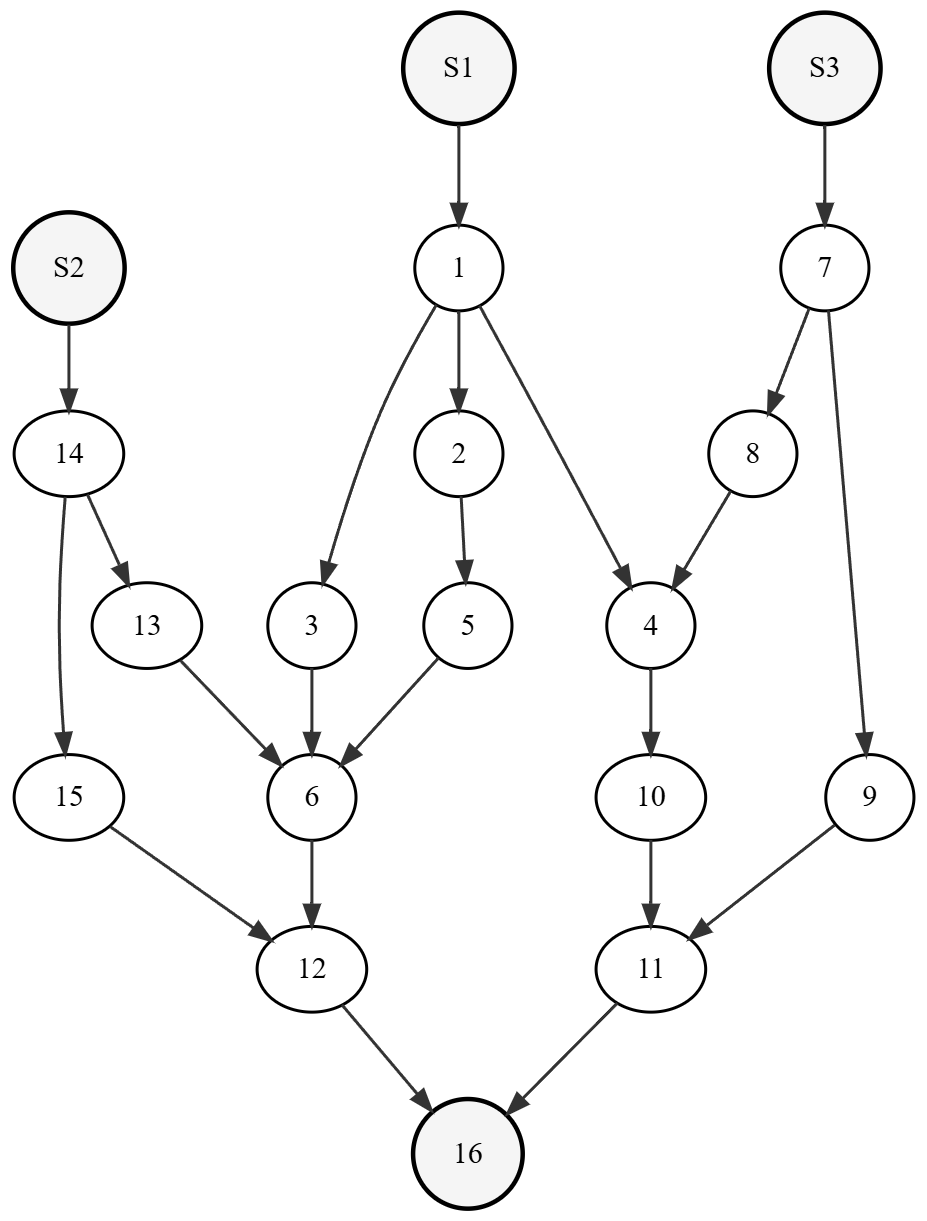
\includegraphics[width=\textwidth]{images/decomp_network/Original Network.png}
    \caption{Original network}
    \label{fig:original}
\end{subfigure}
\quad
\begin{subfigure}[b]{0.21\textwidth}
    \centering
    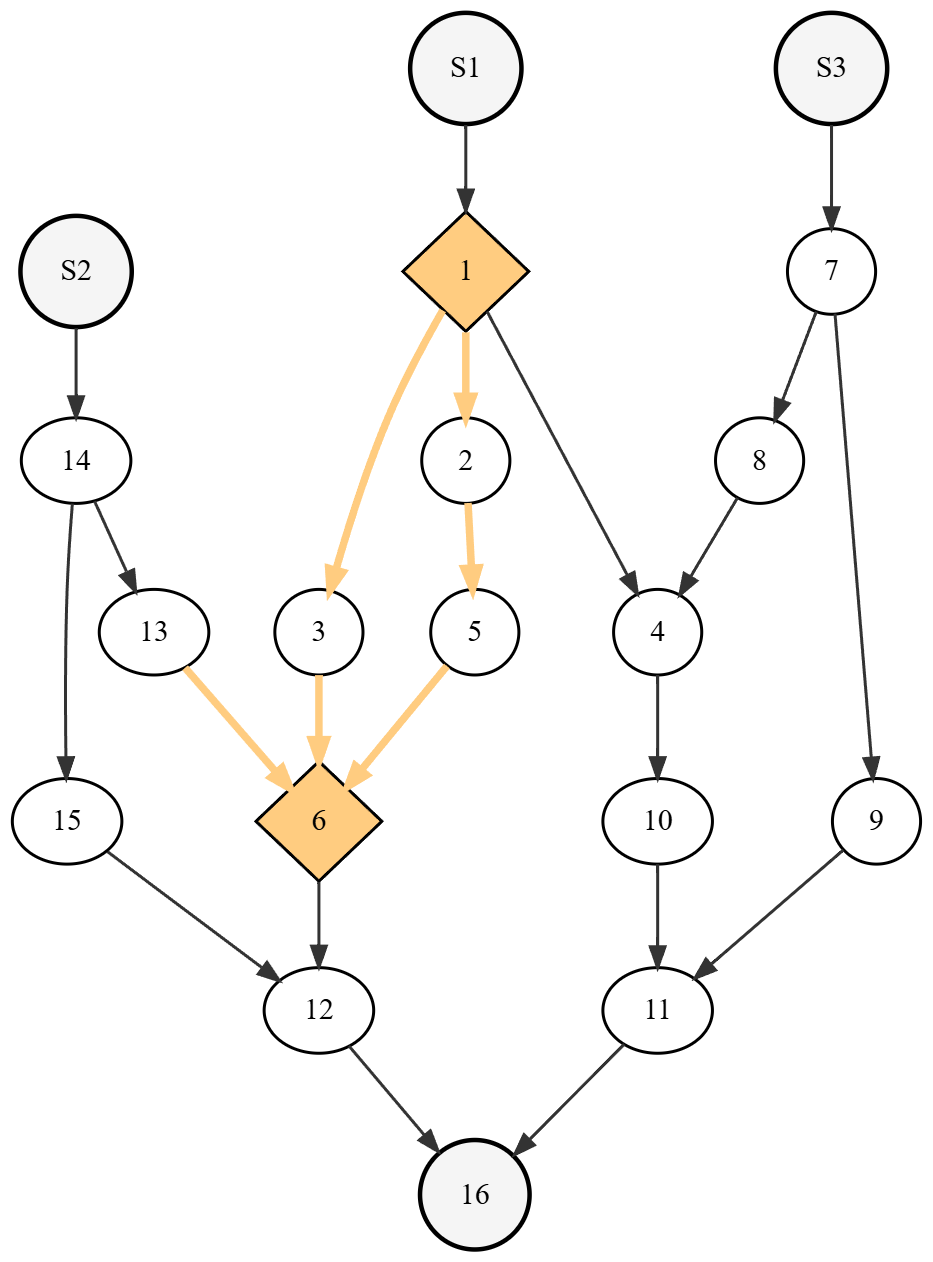
\includegraphics[width=\textwidth]{images/decomp_network/Diamond D1.png}
    \caption{Diamond $D_1$: $1 \rightarrow 6$}
    \label{fig:d1_identify}
\end{subfigure}
\quad
\begin{subfigure}[b]{0.21\textwidth}
    \centering
    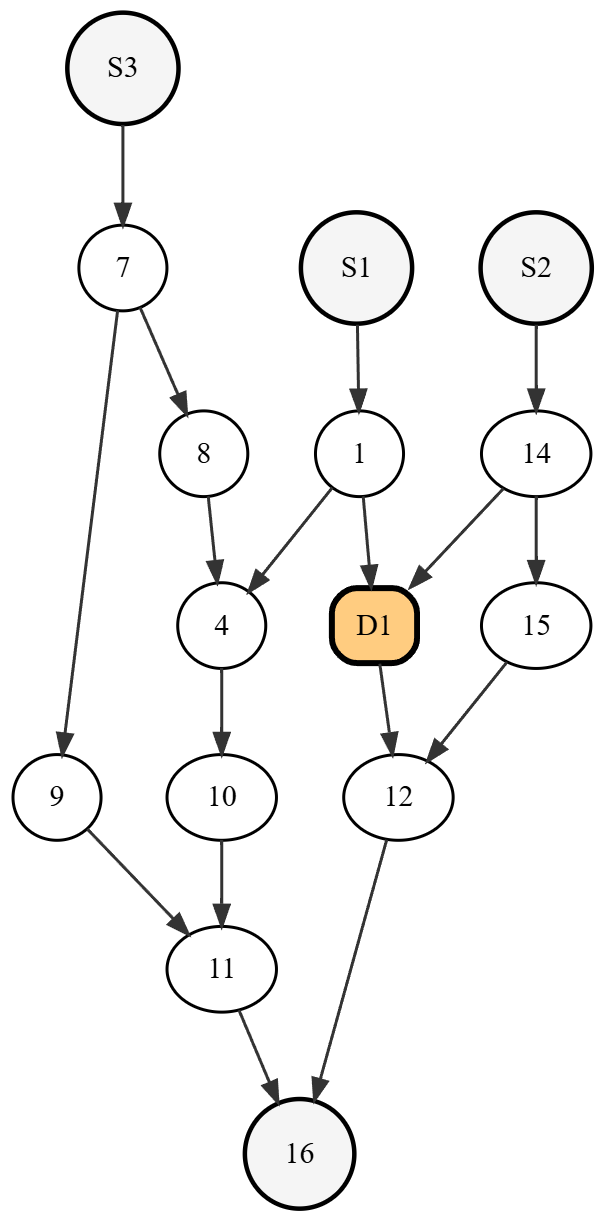
\includegraphics[width=\textwidth]{images/decomp_network/D1 supernode.png}
    \caption{After $D_1$ replacement}
    \label{fig:d1_replace}
\end{subfigure}
\quad
\begin{subfigure}[b]{0.21\textwidth}
    \centering
    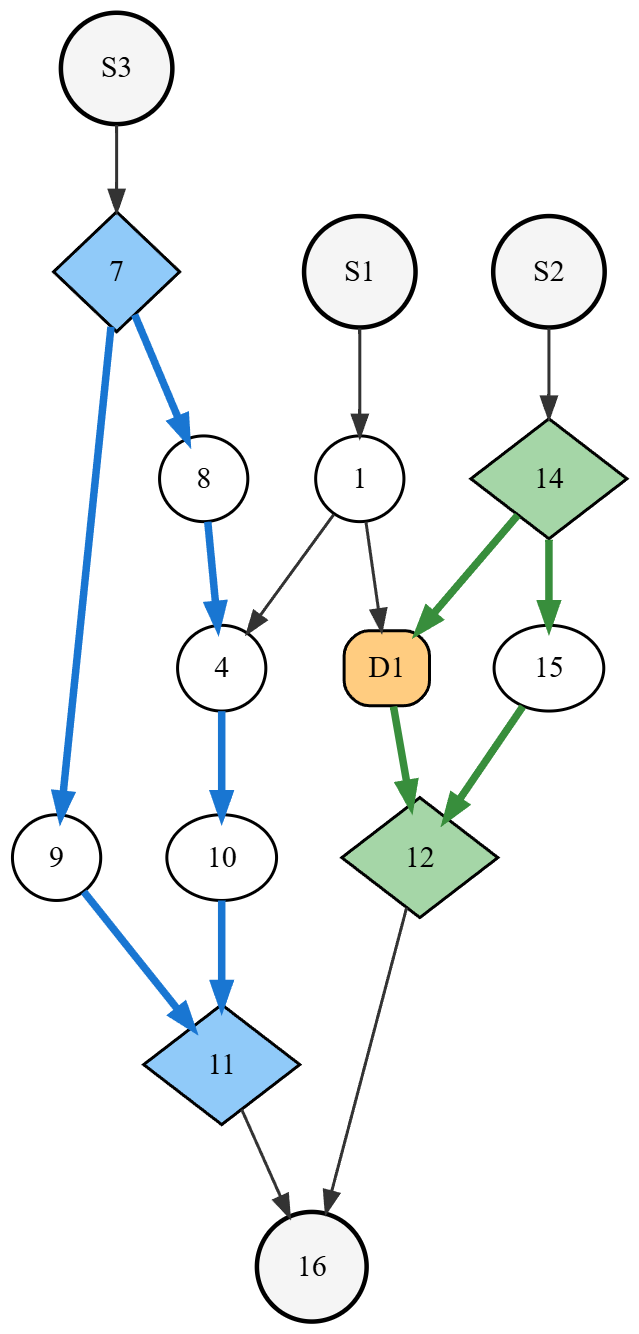
\includegraphics[width=\textwidth]{images/decomp_network/Diamonds D2 and D3.png}
    \caption{Diamonds $D_2$: $7 \rightarrow 11$, $D_3$: $14 \rightarrow 12$}
    \label{fig:d2_d3_identify}
\end{subfigure}

\smallskip

\hspace*{\fill}
\begin{subfigure}[b]{0.25\textwidth}
    \centering
    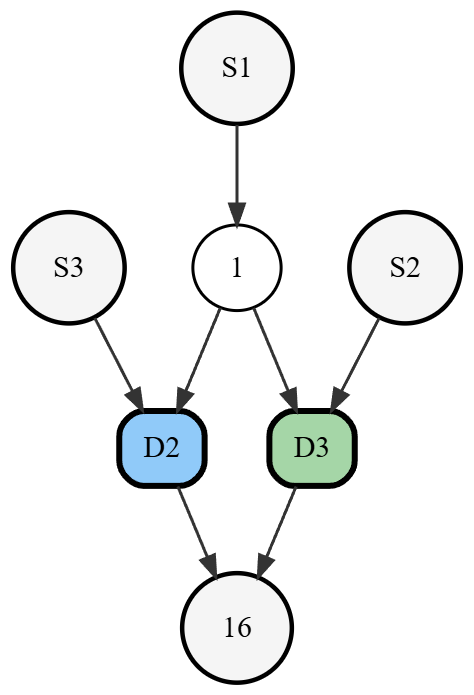
\includegraphics[width=\textwidth]{images/decomp_network/D2 and D3 supernode.png}
    \caption{After $D_2$ and $D_3$ replacement}
    \label{fig:d2_d3_replace}
\end{subfigure}
\hspace*{\fill}
\begin{subfigure}[b]{0.25\textwidth}
    \centering
    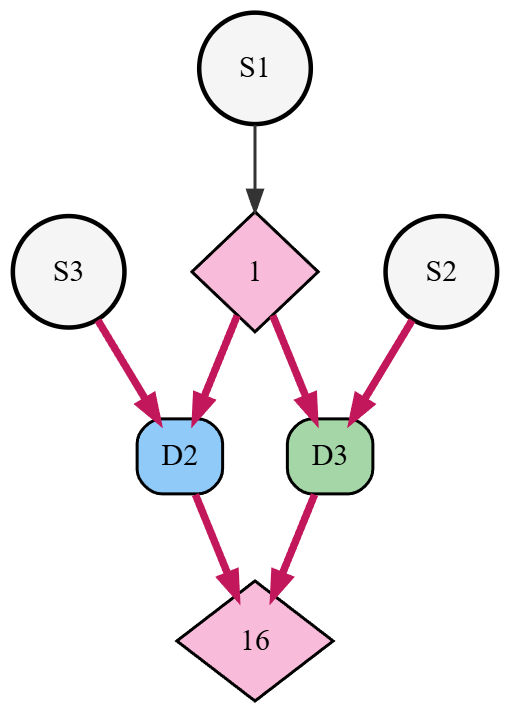
\includegraphics[width=\textwidth]{images/decomp_network/Diamond D4.png}
    \caption{Final diamond $D_4$: $1 \rightarrow 16$}
    \label{fig:d4_identify}
\end{subfigure}
\hspace*{\fill}
\begin{subfigure}[b]{0.25\textwidth}
    \centering
    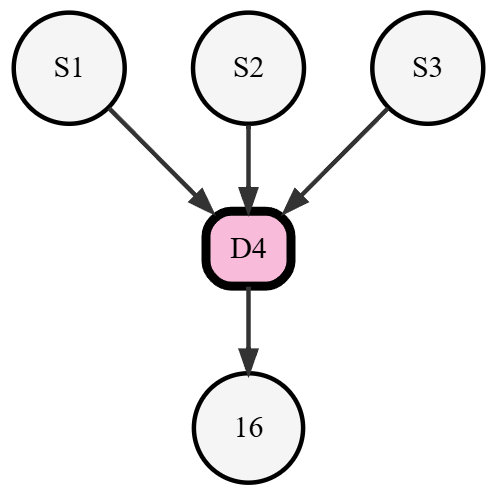
\includegraphics[width=\textwidth]{images/decomp_network/D4 supernode.png}
    \caption{Final decomposition}
    \label{fig:final}
\end{subfigure}
\hspace*{\fill}

\caption{Progressive diamond decomposition in a nested reconvergent network.}
\label{fig:progressive_decomposition}
\end{figure}

\subsubsection{Tracing the example of Figure~\ref{fig:progressive_decomposition}}\label{sec:worked}

The network of Figure~\ref{fig:progressive_decomposition} has three sources and thirteen further nodes; every non-source node has intrinsic reliability $0.9$ and every edge has transmission probability $0.9$, as in Section~\ref{sec:simple_example}. Node 6 has three parents, 3, 5, and 13, but only 3 and 5 trace back to the shared fork 1; the third, 13, traces back through node 14 to a different source and carries no dependency on the other two. IPA therefore does not condition node 6 on a joint state of three variables: it resolves $\{3,5\}$ as diamond $D_1$ (fork 1), then combines the result with node 13's independent signal by the ordinary union rule of Section~\ref{sec:IPA} (Lemma~\ref{lem:factorisation}). Node 4, by contrast, is a join with no diamond at all: its parents 1 and 8 share no common ancestor, so IPA applies the closed-form independent update directly (Section~\ref{sec:IPA}) and never conditions on anything there.

$D_1$ is resolved first, since node 6 is reached before nodes 11, 12, and 16 in topological order. Fork 1 has $b(1)=0.81$; conditional on 1 being reachable, the union of paths through 3 and 5 has probability $\psi_{D_1}(1)=0.8890228$, and conditional on 1 being unreachable no signal can reach 6 through either path, so $\psi_{D_1}(0)=0$. Combining this with node 13's independent signal gives $b(6)=0.7968435$. Diamonds $D_2$ (fork 7, join 11) and $D_3$ (fork 14, join 12) do not depend on $D_1$ or on each other and are resolved the same way, each conditioning on its own fork. The reduced graph then has a single outer diamond, $D_4$: fork 1 again, but now covering join 16 through the two already-resolved supernodes at 11 and 12. Fork 1 is conditioned on a second time here, in a different context from $D_1$, and the two resolutions are kept as distinct stored sub-problems (Section~\ref{sec:identification}) because they cover different edges. Table~\ref{tab:worked} lists all four resolutions; the final belief is $b(16)=0.8061491$, and each step was checked independently by exhaustive path enumeration of its own sub-network.

\begin{table}[ht]
\centering\small
\caption{Trace of the four diamond resolutions in Figure~\ref{fig:progressive_decomposition}. $w=P(\mathcal{R}_f{=}1)$; $\psi(1),\psi(0)$ are the conditional signal probabilities at the join given the fork reachable or unreachable, before the join's own reliability is applied.}
\label{tab:worked}
\begin{tabular}{lcccccc}
\toprule
Diamond & Join & Fork & Group & $w$ & $\psi(1)$, $\psi(0)$ & $b(\text{join})$\\
\midrule
$D_1$ & 6  & 1 & \{3,5\} + 13 (indep.) & 0.81 & 0.8890228,\ 0 & 0.7968435\\
$D_2$ & 11 & 7 & \{10,9\}              & 0.81 & 0.8937451,\ 0.4782969 & 0.7333289\\
$D_3$ & 12 & 14 & \{6,15\}             & 0.81 & 0.9318600,\ 0.5832879 & 0.7790682\\
$D_4$ & 16 & 1 & \{12,11\}             & 0.81 & 0.9139431,\ 0.8180383 & 0.8061491\\
\bottomrule
\end{tabular}
\end{table}

\subsubsection{Identification of stored sub-problems}\label{sec:identification}

Algorithm~\ref{alg:identify} gives the identification procedure itself, run at each join whose parent signals are dependent. It partitions the join's parents into independent ancestry-groups (Lemma~\ref{lem:factorisation}), finds each group's covering fork, and recurses into nested diamonds under an extended context — this is the recursive partition-and-recurse step that Algorithm~\ref{alg:ipa}'s propagation loop invokes in a single line (``identify reconvergent structures affecting $v$''). A node is excluded from a conditioning set only when it is provably degenerate: fixed at prior exactly $0$, or fixed at exactly $1$ \emph{and} a graph source. Excluding any other prior-$1$ node is unsound here — it would silently drop a real diamond whenever every prior in the network happens to equal $1$, which is exactly the input convention of the benchmark grid network of Section~\ref{sec:grid}.

\begin{algorithm}[h]
\caption{Diamond identification at a join node (recursive, factorised)}
\label{alg:identify}
\begin{algorithmic}[1]
\REQUIRE join node $v$, outer conditioning context $E$ (initially $\emptyset$)
\ENSURE independent conditioning groups for $v$, each with its diamond subgraph and conditioning set
\FOR{each parent $p \in \text{Pa}(v)$}
    \STATE compute $\text{infl}(p;E) = (\{p\}\cup\text{anc}(p))\setminus E$ \COMMENT{Eq.~\eqref{eq:infl}}
\ENDFOR
\STATE partition $\text{Pa}(v)$ into groups $G_1,\ldots,G_m$ by union--find: $p,p'$ share a group iff $\text{infl}(p;E)\cap\text{infl}(p';E)\neq\emptyset$ \COMMENT{Lemma~\ref{lem:factorisation}}
\FOR{each group $G_k$}
    \STATE $f_k \gets$ the topologically-highest fork covering $\geq2$ members of $G_k$ (or the case where one member is an ancestor of another)
    \IF{no such fork exists}
        \STATE members of $G_k$ contribute as ordinary non-diamond parents (Section~\ref{sec:IPA})
    \ELSE
        \STATE relevant nodes $\gets \{v\}\cup G_k\cup\text{anc}(G_k)$; induced edges $\mathcal{E}_{D_k} \gets$ edges among relevant nodes not crossing into $E$'s already-fixed context
        \STATE conditioning set $C_k \gets \{f_k\}\cup(E\cap V(\mathcal{E}_{D_k}))$; key $\gets \mathrm{hkey}(D_k)=(\mathcal{E}_{D_k},C_k)$ \COMMENT{Eq.~\eqref{eq:hkey}}
        \IF{a diamond with this key is already resolved}
            \STATE reuse its stored conditional map $\psi_{D_k}$
        \ELSE
            \STATE recurse into $D_k$'s own join nodes with context $E\cup\{f_k\}$, then resolve and store $\psi_{D_k}$
        \ENDIF
    \ENDIF
\ENDFOR
\RETURN groups $G_1,\ldots,G_m$, each with its conditioning set and conditional map
\end{algorithmic}
\end{algorithm}

A resolved diamond is identified for reuse by its edge list together with the conditioning context it was resolved under, not by its edge list alone. The same edge list can arise from a fork that is free or already fixed by an outer context $E$, because cutting the incoming edges of an already-fixed node changes nothing in the induced subgraph; the two occurrences are nonetheless different sub-problems, since Lemma~\ref{lem:invariance} requires the outer context to fix no variable internal to the diamond. IPA keys each stored diamond $D$, with edge list $\mathcal{E}_D$ and covering fork $f$, on
\begin{equation}
\mathrm{hkey}(D) = \bigl(\mathcal{E}_D,\ \{f\}\cup(E\cap V(\mathcal{E}_D))\bigr),
\label{eq:hkey}
\end{equation}
the edge list together with the new fork and whichever already-fixed forks from the outer context appear among the diamond's own endpoints $V(\mathcal{E}_D)$. Two occurrences of the same edge list under different outer contexts receive different keys and are resolved, and cached, separately; identical sub-problems are resolved once. A conditioning node already fixed by an outer context contributes only one term to the state enumeration of Section~\ref{sec:numerical}, not two, so nesting further levels of context does not double the enumeration already performed at each level.

\subsection{Complexity and Relation to Established Exact Methods}\label{sec:complexity}

IPA's cost admits an exact per-instance expression. Let the recursion of Section~\ref{sec:procedure} resolve diamonds $d=1,\ldots,M$, counting nested resolutions, with conditioning sets $C_d$ and internal edge sets $E_d$. The work performed is
\begin{equation}
W=\sum_{d=1}^{M}2^{|C_d|}\cdot O(|E_d|),
\label{eq:work}
\end{equation}
since each diamond is resolved by enumerating the $2^{|C_d|}$ states of its conditioning set, and each state requires a propagation over the diamond's internal structure. Every term of \eqref{eq:work} is available before enumeration begins, because identification produces the conditioning sets before any state is enumerated; $W$ is a sound a-priori \emph{upper bound} on the cost of an analysis, computable in advance for a given network. This bound is not the realised cost: memoisation under \eqref{eq:hkey} reduces the work performed to the number of distinct conditional sub-problems encountered. The factorisation of Lemma~\ref{lem:factorisation} reduces the exponents themselves in favourable cases: at a fan-in of $k$ independent branches, from $2^k$ states to a number linear in $k$, without changing the worst-case class.

\paragraph{Relation to cutset conditioning and junction trees} Section~\ref{subsec:relatedworks} positions IPA as a specialisation of cutset conditioning~\cite{pearl_probabilistic_1988}. Classical cutset conditioning selects a single global cutset whose state enumeration renders the whole network singly connected, at cost exponential in the cutset size. IPA identifies, at each reconvergence it visits, a local separating set of the parents' shared ancestry (Lemma~\ref{lem:separator}), conditions on it, and recurses, so the realised cost is a sum of local exponentials, not one global exponential. Tree-structured regions of the network are traversed by the closed-form updates of Section~\ref{sec:IPA} at linear cost, and Lemma~\ref{lem:factorisation} prevents joint conditioning over forks that are independent given the current context. The maximum conditioning-set size on a network is bounded by the size of the largest set of mutually entangled shared ancestors, itself bounded by the treewidth of the network. IPA sits in the same parametric complexity class as the junction-tree algorithm~\cite{lauritzen_local_1988} and a well-ordered binary decision diagram: all are exact and fixed-parameter tractable in the relevant width, and none escapes the \#P-hardness of the underlying problem. Section~\ref{sec:comparison} reports a measured comparison of conditioning-set size against decision-diagram size across the validation corpus.

\paragraph{Adversarial structure} Two constructed families probe the two ends of this cost. The family $\mathrm{fanin}\text{-}k$ consists of $k$ structurally independent forks that each reconverge, on their own branch, at a single shared join; since no two forks share ancestry, Lemma~\ref{lem:factorisation} conditions each one separately, and identification resolves exactly $2k{+}1$ sub-problems for every $k$ tested. The family $\mathrm{mesh}\text{-}w$ is the opposite extreme: a width-$w$ reconvergent lattice with no independent partition, a single fully correlated block on which factorisation does not apply, so the conditioning-set size and the realised work both grow with $w$. Table~\ref{tab:adversarial} reports both families against an independent decision-diagram method built under dynamic variable reordering: independent structure is resolved at a cost linear in the fan-in, while correlated structure pays the full width-exponential cost of \eqref{eq:work}. A real published benchmark circuit family, assigned the same worst-case input convention, is examined in Section~\ref{sec:adversarial}.

\begin{table}[ht]
\centering\small
\caption{Complexity on the two adversarial families: realised sub-problems for IPA (with factorisation) against a sifted reduced-ordered binary decision diagram, in operation-count and wall-clock terms.}
\label{tab:adversarial}
\begin{tabular}{lrrrrr}
\toprule
Family & param & IPA sub-problems & diagram nodes & IPA time & diagram time\\
\midrule
fan-in-$k$ & 8  & 17 & 474 & $<$1\,ms & $\sim$1--2\,s\\
fan-in-$k$ & 16 & 33 & 802 & $<$1\,ms & $\sim$1--2\,s\\
mesh-$w$   & 4  & 20{,}603 & 700 & 0.37\,s & 1.19\,s\\
mesh-$w$   & 5  & 170{,}001 & 805 & 3.9\,s & 1.2\,s\\
mesh-$w$   & 8  & 3{,}895{,}252 & 2{,}621 & 159.5\,s & 2.9\,s\\
mesh-$w$   & 9  & 5{,}426{,}417 & 3{,}335 & 5925\,s & 3.8\,s\\
\bottomrule
\end{tabular}
\end{table}

At $w{=}9$ the sub-problem count grows by only $1.39\times$ over $w{=}8$ (3{,}895{,}252 to 5{,}426{,}417) while IPA's wall-clock time grows by $37\times$ (159.5\,s to 5925\,s); $w{=}10$ exceeded a 180-second-per-step time budget during identification and was not completed. The sub-problem count of \eqref{eq:work} tracks realised work only up to a point: at the largest conditioning-set sizes reached in this family, memory pressure within individual sub-problems begins to dominate wall-clock cost before it is reflected in the sub-problem count itself, and the decision diagram's wall-clock cost — already lower at every mesh-$w$ point tested — pulls further ahead than the sub-problem-count comparison alone would suggest.

\paragraph{Applicability beyond source-to-node reachability} Cutset conditioning already applies to general Bayesian-network inference: IPA specialises that method to source-to-node reachability, and this specialisation does not generalise back to arbitrary probabilistic graphical models. Its closed-form update rules, the independent-union combination of parent signals and the context-keyed supernode cache, are derived for the monotone reachability structure of \eqref{eq:reach_indicator} and do not carry over directly to a Bayesian network with arbitrary conditional probability tables. What transfers is the width-governed complexity class established above. This distinction also bears on the imprecise propagation of Section~\ref{subsec:impreciseinputs}: for classical, precise Bayesian networks, bounded treewidth guarantees polynomial exact inference, but this guarantee does not survive the move to imprecise, credal parameters, where bounded-treewidth inference remains NP-hard in general~\cite{maua_thirty_2020}, and the only known tractable relaxation is an approximation scheme; no known exact one exists for that case~\cite{fagiuoli_2u_1998}. IPA's width-governed \emph{exact} imprecise result (Section~\ref{sec:imprecise}) is specific to the monotone arithmetic structure of the reachability problem and the explicit diamond-conditioning construction; it does not imply that general credal-network inference could be made exact at the same cost.

\subsection{Numerical Realisation}\label{sec:numerical}

IPA is implemented in Julia as part of the \texttt{InfoPropFramework.jl} package and the standalone library \texttt{InformationPropagationAnalysis.jl}, with diamond identification exposed in \texttt{DiamondDecompositionModule} and belief propagation in \texttt{ProbabilityPropagationModule}, following Section~\ref{sec:IPA} and Algorithm~\ref{alg:ipa}. The propagation flow is type-parametric,
\[
T <: \mathrm{Union}\{\texttt{Float64}, \texttt{Interval}, \texttt{pbox}\},
\]
with one core engine shared across all three representations and type-specific dispatch through common arithmetic helpers (addition, multiplication, complement).

Multi-parent updates are evaluated in the product form $1-\prod_i(1-p_i)$. This is equivalent under independence to the alternating inclusion--exclusion sum, but the product form is numerically stable and avoids the spurious widening the alternating sum introduces for interval-valued inputs. At a resolved diamond, beliefs are computed by enumerating the states of its \emph{active} conditioning set: a conditioning node whose contextual belief is already pinned to $0$ or $1$ by an outer conditioning contributes only one term, not two, matching \eqref{eq:hkey}'s treatment of already-fixed forks, and never changes the result, since the dropped state carries zero weight. Two caches support this: one keyed on $\mathrm{hkey}(D)$ (Section~\ref{sec:identification}) avoids re-identifying the same diamond, and a second, keyed on a diamond's edge list together with the node priors of a given conditioning state, avoids recomputing a state's belief when the identical sub-problem recurs under a different diamond or context.

For interval inputs, each conditioning state is evaluated at the corner states of the conditioning bounds, and the result is enclosed in an interval envelope; Section~\ref{sec:imprecise} shows this yields the exact range, by the monotonicity of \eqref{eq:reach_indicator}. For probability-box inputs, recombining a diamond's two conditional branches is a convex combination of two dependent random quantities, not an independent sum: a flat weighted sum of the branch distributions, exact for the point-valued and interval cases, is unsound for probability boxes, since it double-counts the shared dependence on the conditioning weight and can return a bound outside $[0,1]$. IPA combines the two branches through the operator of Williamson and Downs~\cite{williamson_probabilistic_1990}, nesting one such combination per conditioning node so that $m$ nested two-way combinations reproduce the $2^m$-state mixture exactly.

This recursive structure is shared across all three input types: the number of conditioning states enumerated per diamond, after the memoisation of Section~\ref{sec:identification}, is the same realised-work quantity reported in Section~\ref{sec:complexity}. What differs is the price paid per resolved state. For point-valued and interval inputs this price is $O(1)$; for probability-box inputs, the conditioning weight is represented at a chosen discretisation level, and each combination integrates over that discretisation via the convolution of Williamson and Downs~\cite{williamson_probabilistic_1990}, at a cost that increases with the discretisation level. Probability-box cost is therefore governed by the same realised sub-problem count as the exact and interval cases, multiplied by a per-state price set by the discretisation level, and Section~\ref{sec:imprecise} reports this cost in those terms, not against network size alone.



\clearpage  % Forces all pending floats to be placed
\section{Case Studies}\label{sec:cases}

This section evaluates IPA in four steps: a benchmark validation on a grid network (Section~\ref{sec:grid}); a corpus-wide validation and cost comparison against an independent exact decision-diagram method (Section~\ref{sec:comparison}); the imprecise-propagation capability (Section~\ref{sec:imprecise}); and an applied case study of a medical drone logistics network for Scotland (Section~\ref{sec:drone}). Section~\ref{sec:adversarial} then examines a real published benchmark family under an adversarial input convention.

Two methodological points hold throughout the section. Every runtime is measured after a warm-up run of the same computation is executed and discarded, so one-off program-initialisation cost is excluded, and the reported time is the minimum of repeated measurements on otherwise idle hardware. All decision-diagram comparisons use CUDD~\cite{somenzi_cudd}, called from the same process and machine as IPA, with dynamic variable reordering enabled unless stated otherwise. Where component reliabilities are widened into intervals or probability boxes for illustration, only components that are not structurally certain are widened: a component fixed at reliability exactly 0 or 1 by the network's own structure is left at that value, since degrading a structural certainty into a synthetic uncertainty would change the problem being analysed.

\subsection{Benchmark Validation on a Grid Network}\label{sec:grid}

\subsubsection{Benchmark setup}

The proposed method and Tong and Tien's directed Probability Propagation Method (dPrPm)~\cite{tong_probability_2019} both compute node reliability in directed acyclic networks by propagating local probability information from upstream to downstream nodes, exploiting the acyclic structure so that upstream dependencies are processed before downstream updates. The two methods differ in how dependencies are represented. dPrPm propagates both marginal and pairwise probabilities and approximates a three-node joint distribution for every edge that introduces a new dependency; this requires storing pairwise probabilities throughout the network, which becomes memory-intensive in large or dense networks. IPA instead identifies reconvergent dependency patterns as diamond structures and resolves them through conditional decomposition (Section~\ref{sec:IPA}). It does not track pairwise relationships: each diamond is decomposed once into a statistically equivalent supernode, and the relevant dependency structure is captured once in that decomposition, not maintained node by node.

To provide a direct benchmark, IPA is applied to the same 16-node directed grid network studied in~\cite{tong_probability_2019}, shown in Figure~\ref{fig:grid_network}. This benchmark contains multiple reconvergent structures while remaining small enough for exact verification by explicit path enumeration. Following~\cite{tong_probability_2019}, all source nodes are assigned prior reliability $1.0$ and all directed edges are assigned transmission probability $0.9$.

\begin{figure}[htbp]
\centering
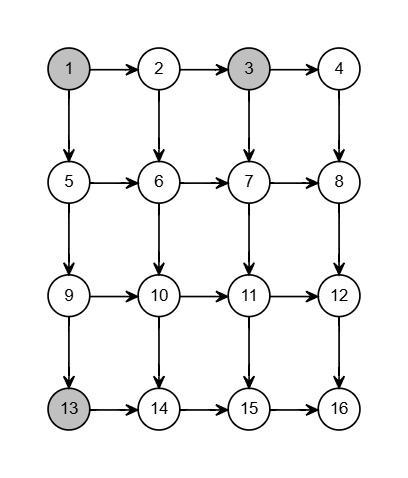
\includegraphics[width=0.8\linewidth, height=8cm]{images/grid_graph.png}
\caption{16-node directed grid network~\cite{tong_probability_2019}. Source nodes 1, 3, and 13 are coloured in grey.}
\label{fig:grid_network}
\end{figure}

\subsubsection{Accuracy results}

Table~\ref{tab:resultcomparison_grid} brings together three independent quantities at every node: the value IPA computes, the value a reduced-ordered binary decision diagram (ROBDD) computes for the same network, and the lower and upper bounds published for dPrPm in~\cite{tong_probability_2019}. IPA and the ROBDD agree to floating-point precision at every node, with a worst disagreement of $1.1\times10^{-16}$; the column reported as exact is therefore not IPA's own output taken on trust, but a value two independent exact methods reach separately. Against that value, the dPrPm bounds coincide everywhere except node 16, where a gap of $0.00048$ remains: the same node the source study itself identifies as the lowest-probability, hardest-to-bound event in the benchmark.

\begin{table}[!ht]
\centering\small
\caption{Node reliabilities on the benchmark grid network ($R_l=0.9$). The exact column is where IPA and an independent ROBDD agree (worst disagreement $1.1\times10^{-16}$); dPrPm lower/upper bounds and gap are as reported in~\cite{tong_probability_2019}, Table 2. Source nodes (1, 3, 13) are fixed at reliability 1 and are not reported as dPrPm bounds in the source study.}
\label{tab:resultcomparison_grid}
\begin{tabular}{ccccc}
\toprule
Node & Exact = IPA & dPrPm lower & dPrPm upper & Gap \\
\midrule
1  & 1.00000000 & -- & -- & -- \\
2  & 0.99000000 & 0.99000 & 0.99000 & 0.00000 \\
3  & 1.00000000 & -- & -- & -- \\
4  & 0.98015430 & 0.98015 & 0.98015 & 0.00000 \\
5  & 0.90000000 & 0.90000 & 0.90000 & 0.00000 \\
6  & 0.99510274 & 0.99510 & 0.99510 & 0.00000 \\
7  & 0.98955925 & 0.98956 & 0.98956 & 0.00000 \\
8  & 0.89060332 & 0.89060 & 0.89060 & 0.00000 \\
9  & 0.98100000 & 0.98100 & 0.98100 & 0.00000 \\
10 & 0.88290000 & 0.88290 & 0.88290 & 0.00000 \\
11 & 0.97734390 & 0.97734 & 0.97734 & 0.00000 \\
12 & 0.97456525 & 0.97457 & 0.97457 & 0.00000 \\
13 & 1.00000000 & -- & -- & -- \\
14 & 0.97946100 & 0.97946 & 0.97946 & 0.00000 \\
15 & 0.98497989 & 0.98498 & 0.98498 & 0.00000 \\
16 & 0.98538853 & 0.98506 & 0.98558 & 0.00048 \\
\bottomrule
\end{tabular}
\end{table}

Table~\ref{tab:computation_comparison_grid} reports the runtime of IPA on this benchmark against the runtime reported for dPrPm. Two caveats attend the comparison. The dPrPm figure is quoted from the source study, obtained in a different implementation environment, so the comparison is indicative only. The dPrPm reference implementation is not publicly available and its authors could not be reached, so the comparison cannot be reproduced independently. The table therefore carries no ROBDD row: a build-time figure for this one network, on its own, would invite exactly the kind of uncontrolled comparison already rejected for dPrPm. The controlled, same-environment cost comparison against the ROBDD, built for every network in the corpus including this one, is reported instead in Section~\ref{sec:comparison} (this network's ROBDD has 290 nodes; Table~\ref{tab:structured}); dPrPm is retained here only as the published point of reference that motivated the benchmark.

\begin{table}[ht]
\centering\small
\caption{Computational performance on the benchmark grid network. IPA figures are machine-specific (measured on the authors' current hardware after a discarded warm-up run) and are reported to characterise order of magnitude, not for cross-machine comparison. The dPrPm runtime is quoted from~\cite{tong_probability_2019} and is indicative only.}
\label{tab:computation_comparison_grid}
\begin{tabular}{lcc}
\toprule
Method & Runtime & Memory \\
\midrule
IPA & 0.910\,ms & 1.74\,MB \\
dPrPm (reported) & 0.32\,s & n/a \\
\bottomrule
\end{tabular}
\end{table}

This benchmark's ROBDD confirmation was also used to stress-test identification beyond the benchmark's own parameterisation, with non-unit node priors and the boundary case in which every node prior equals one; two edge-case identification errors were found this way and corrected, and the corrected version is the one validated across the full corpus of Section~\ref{sec:comparison}. Neither error affects the benchmark table above, which stands as originally computed.

\subsection{Validation and Cost Comparison Against an Exact Decision-Diagram Method}\label{sec:comparison}

% TODO (parity check): this sentence stacks the 129-graph corpus (Table~\ref{tab:corpus}) with the
% six-family timing corpus (Table~\ref{tab:interval_timing}) and the named structured/real networks
% (Table~\ref{tab:structured} + Memphis/Berlin/Net3) without stating whether these are disjoint,
% overlapping, or a combined total -- "counterexample" and "random n=25" appear in more than one of
% these groups. "larger random networks up to 50 nodes" has no traced source in this session's audit
% (tab:corpus tops out at n=25). Needs attribution/re-scoping once traced -- see
% NUMERIC_PARITY_AUDIT_HANDOVER.md.
To address the breadth of validation, IPA was compared against an independent exact method, a reduced-ordered binary decision diagram (ROBDD) with dynamic variable reordering, across a corpus of 129 random and mutated DAGs (10 to 28 nodes, densities 0.14--0.42), six topological families (multi-source, grid/lattice, layered, bridge, series--parallel, complete), larger random networks up to 50 nodes, and several structured and real-world networks: a gas distribution network (Memphis Light, Gas and Water), a metropolitan transit network (Berlin), and a water distribution benchmark (EPANET Net3), in addition to the power distribution and drone logistics networks studied in detail in Sections~\ref{sec:grid} and~\ref{sec:drone}. Table~\ref{tab:structured} reports representative structured and real networks in detail, and Table~\ref{tab:corpus} summarises the random corpus by family.

Every network in the corpus was evaluated by both methods; the worst per-node disagreement observed anywhere is $1.1\times10^{-16}$, for both perfect and imperfect component reliabilities. Structural exactness was additionally verified against 17 published Bayesian-network benchmark topologies (bnlearn.com/bnrepository), ranging from 8 to 1{,}041 nodes. Component reliabilities on these 17 networks are illustrative, not decision-relevant: the check demonstrates breadth of topology and scale, not a claim about the systems the benchmarks originally model.

\begin{table}[ht]
\centering\small
\caption{Exactness and complexity of IPA on named structured networks, against the exact ROBDD oracle. Root D.\ and uniq.\ D.\ are the numbers of root and unique diamond structures identified; $|C|_{\max}$ is the largest conditioning set; ROBDD is the node count under dynamic reordering; $|\Delta|_{\max}$ is the worst per-node deviation of IPA from the exact ROBDD reliability.}
\label{tab:structured}
\begin{tabular}{lrrrrrrrl}
\toprule
Network & $|V|$ & $|E|$ & src & root D. & uniq.\ D. & $|C|_{\max}$ & ROBDD & $|\Delta|_{\max}$ \\
\midrule
power network      & 23 & 27 & 3 &  5 &   9 &  3 &  384 & $8.3\times10^{-17}$ \\
grid (benchmark)   & 16 & 24 & 3 &  8 &  39 &  7 &  290 & $1.1\times10^{-16}$ \\
Karl network       & 26 & 74 & 1 & 18 & 145 & 11 & 1921 & $5.6\times10^{-17}$ \\
counterexample-n15 & 15 & 23 & 1 &  4 &  13 &  4 &  323 & $5.6\times10^{-17}$ \\
\bottomrule
\end{tabular}
\end{table}

\begin{table}[ht]
\centering\small
\caption{Random and mutated DAG corpus (129 graphs), summarised by family. Random DAGs are generated per family at edge probability $p\in\{0.10,0.15,0.20\}$ and eight seeds; mutant-n28 is a base $n=28$ DAG under $+5/-2$ edge mutations. Every graph in every family is exact against the ROBDD oracle ($|\Delta|_{\max}\le1.1\times10^{-16}$ across the whole corpus). Naive blow-ups are builds exceeding $2.5\times10^{6}$ ROBDD nodes under a naive (topological) variable order, all resolved by dynamic reordering.}
\label{tab:corpus}
\begin{tabular}{lrrrrrr}
\toprule
Family & \#graphs & $|V|$ & $|E|$ & density & med.\ ROBDD & naive blow-ups \\
\midrule
random-n10  & 24 & 10 & 12--18 & 0.27--0.40 &   80 & 0 \\
random-n12  & 24 & 12 & 15--28 & 0.23--0.42 &  197 & 0 \\
random-n15  & 24 & 15 & 21--35 & 0.20--0.33 &  450 & 0 \\
random-n20  & 24 & 20 & 31--50 & 0.16--0.26 & 1164 & 0 \\
random-n25  & 24 & 25 & 42--73 & 0.14--0.24 & 3119 & 9 \\
mutant-n28  &  8 & 28 & 62     & 0.16       & 2562 & 6 \\
counterexample &  1 & 15 & 23  & 0.22       &  323 & 0 \\
\bottomrule
\end{tabular}
\end{table}

The comparison also quantifies cost. For each network we report the maximum conditioning-set size $|C|_{\max}$ encountered by IPA, its realised number of distinct conditional sub-problems, and the ROBDD node count under dynamic reordering. As anticipated in Section~\ref{sec:complexity}, $|C|_{\max}$ tracks the logarithm of the ROBDD size across the corpus (Figure~\ref{fig:width}), confirming that the two methods are governed by the same structural width. The realised work of the two methods is of the same order, and neither dominates: on some networks IPA resolves fewer sub-problems than the diagram has nodes (42 against 323 on the counterexample network; 142 against 759 on the complete 8-node network), on others more (1961 against 1043 on a layered network). No family in the corpus favours IPA for exact point-valued computation: its value rests on the imprecise-propagation capability of Section~\ref{sec:imprecise}, not on a smaller exact state space.

\begin{figure}[ht]
\centering
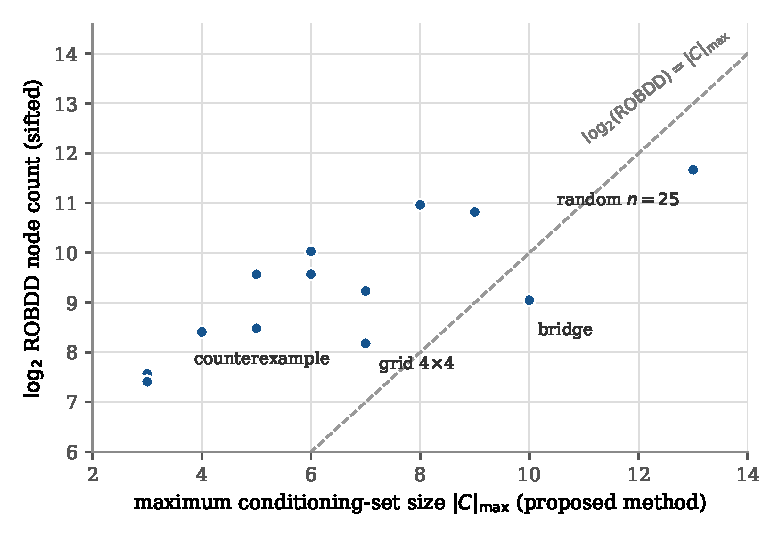
\includegraphics[width=0.75\linewidth]{images/width_correlation.pdf}
\caption{IPA's maximum conditioning-set size against the logarithm of the sifted ROBDD node count, across the complexity-validation networks. Both quantities measure the same structural width; neither method dominates.}
\label{fig:width}
\end{figure}

\subsection{Imprecise Reliability Propagation}\label{sec:imprecise}

The results so far establish that IPA matches a well-ordered decision diagram on exact point-valued reliability at comparable cost. This section presents the capability that separates the two: the propagation scheme accepts interval- and p-box-valued component reliabilities directly (Section~\ref{subsec:impreciseinputs}).

\subsubsection{Interval-valued reliabilities: exact and fast}\label{sec:interval}

Because $b(v)$ is non-decreasing in every component reliability (Section~\ref{sec:model}), its exact range over interval inputs is attained at the two extreme corners of the input box: the lower bound when every component takes its lower reliability, the upper bound when every component takes its upper reliability. This was verified across the full corpus of Section~\ref{sec:comparison} by comparing the propagated interval against the decision-diagram evaluation at both corner inputs: the worst discrepancy in either bound is of order $10^{-16}$. Interval propagation that ignores reconvergent dependence, by contrast, over-widens the range by up to $0.45$ across the corpus, showing that the conditioning machinery of Section~\ref{sec:decomp} is as necessary for sound imprecise propagation as it is for exact point values.

The interval computation is also fast. For a one-shot query (given a network, produce the interval reliability), IPA completed faster than the decision-diagram route to the same answer (build the diagram once, evaluate at both corner inputs) on every one of eight corpus families tested, by factors ranging from $3.9$ to $99.9$ (Table~\ref{tab:interval_timing}). This claim is scoped to the one-shot cost, in which the diagram's construction cost counts against it; a workload that amortises a single construction across many repeated queries on a fixed network is a different scenario, not tested here, and could favour the diagram route instead.

\begin{table}[ht]
\centering\small
\caption{One-shot interval reliability: IPA against the decision-diagram route (build once, evaluate at both corner inputs), warm-measured. IPA is faster on every family tested; the comparison is scoped to one-shot queries.}
\label{tab:interval_timing}
\begin{tabular}{lrrrrrr}
\toprule
Network & $|V|$ & $|E|$ & ROBDD & IPA (ms) & ROBDD route (ms) & ratio \\
\midrule
counterexample       & 15 & 23 &  323 &  0.819 &  44.603 & 54.5 \\
multi-source         & 25 & 57 & 5622 & 22.422 & 175.497 &  7.8 \\
grid $4\times4$      & 16 & 21 &  248 &  0.517 &  51.654 & 99.9 \\
layered $4\times6$   & 23 & 35 &  484 &  4.619 &  52.075 & 11.3 \\
bridge               & 16 & 25 &  529 & 11.571 &  48.515 &  4.2 \\
series--parallel     & 23 & 32 &  215 &  2.429 &  57.304 & 23.6 \\
complete-8           &  8 & 28 &  685 &  1.537 &  49.466 & 32.2 \\
random $n{=}25$      & 25 & 53 & 4146 & 27.844 & 107.875 &  3.9 \\
\bottomrule
\end{tabular}
\end{table}

\subsubsection{Probability-box reliabilities: guaranteed distributional bounds}\label{sec:pbox}

At a join resolved by conditioning with p-box inputs, the belief is a convex combination $W\cdot A+(1-W)\cdot B$, where $W$ is the uncertain probability of the conditioning state and $A,B$ are the uncertain conditional beliefs of the two branches. $A$ and $B$ are functions of shared upstream reliabilities and are therefore dependent; treating the combination as an independent sum is unsound and can assign probability mass outside $[0,1]$. IPA instead integrates over the distribution of $W$, combining the branch distributions at each weight level, with the branch dependence bounded by the Fr\'echet--Hoeffding inequalities~\cite{williamson_probabilistic_1990}. Soundness of the resulting bounds is inherited from that classical result: the computed pair of distribution functions encloses the true distribution of the node reliability under any dependence between the branches. A tighter variant restricts the dependence bound to non-negative dependence, motivated by both branches being non-decreasing functions of the shared upstream reliabilities and so unable to be negatively dependent; this variant produced no soundness violation in any validation configuration tested (dozens of topology, input-shape, and uncertainty-width combinations, each checked against Monte Carlo ground truth), but a general proof of its soundness under partial dependence information of this kind is not available and is future work. Every headline claim in this paper uses only the provable Fr\'echet-based bound.

Bound tightness, as distinct from soundness, depends on the network's structure. Across a sweep of input-distribution shapes, uncertainty widths, and reconvergence regimes on the benchmark grid network of Section~\ref{sec:grid}, the certified band ranged from approximately $0.18$ of the unit range under high-reliability, weakly reconvergent conditions to approximately $0.70$ under strongly reconvergent, fully uncertain conditions, with zero soundness violations across the sweep (Figure~\ref{fig:envelope}). Reconvergence depth combined with input uncertainty drives tightness; the shape of the input distribution is secondary.

\begin{figure}[ht]
\centering
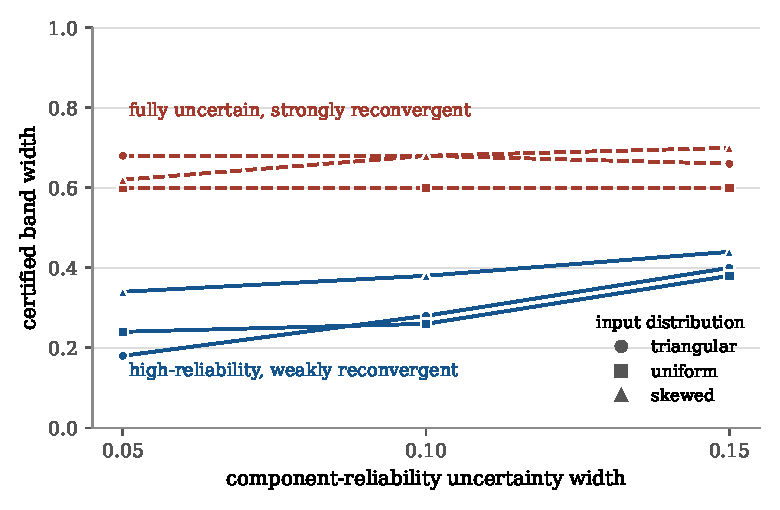
\includegraphics[width=0.8\linewidth]{images/envelope.pdf}
\caption{Tightness envelope of the certified p-box bound on the benchmark network: band width against component-reliability uncertainty width, for three input-distribution shapes and two reconvergence regimes. Soundness holds in every configuration; only tightness varies, and it is driven by the regime, not the input shape.}
\label{fig:envelope}
\end{figure}

Computational cost is a controllable dial. Interval propagation costs a small constant factor over point-valued propagation (about $1.8$ in our measurements: $0.465$\,ms against $0.819$\,ms on the counterexample-n15 network of Table~\ref{tab:structured}), while p-box propagation grows with the discretisation level of the distribution bounds: $1.54$\,s, $8.68$\,s, $51.02$\,s, and $339.02$\,s at $25$, $50$, $100$, and $200$ levels respectively on that same counterexample network, each measured as a single propagation in its own fresh process (a shared warm process inflates later, larger measurements, so one clean process per measurement is used throughout this paper). The resulting exponent is approximately $2.6$ over this range and increases toward its upper end; propagation beyond $200$ levels is impractical on this network and is not used. We therefore state bound tightness always at the discretisation level used, and make no claim that distributional propagation is cheap: it is controllable, with rigorous bounds at every setting.

The same realised-work quantity that governs Float64 and interval cost (Section~\ref{sec:complexity}) also governs p-box cost, at a fixed discretisation level. Figure~\ref{fig:pbox_cost} plots p-box propagation time at steps$=50$ against the realised sub-problem count already reported for the exact and interval comparison, across 14 networks spanning a $141\times$ range in that count. The relationship is close to linear on log-log axes, with time per sub-problem clustered within roughly $0.14$--$0.26$\,s throughout; the raw conditioning-set-width bound $2^{|C|}$, by contrast, does not correlate this cleanly, since two networks with similar bounds can differ substantially in realised sub-problems after memoisation.

\begin{figure}[ht]
\centering
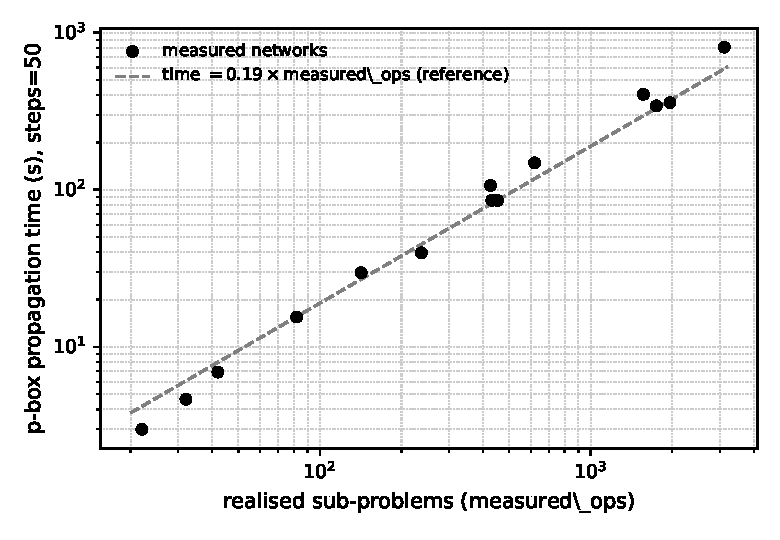
\includegraphics[width=0.75\linewidth]{images/pbox_cost.pdf}
\caption{p-box propagation time at a fixed discretisation level (steps$=50$) against the realised sub-problem count (measured\_ops) already reported for the exact/interval cost comparison (Section~\ref{sec:complexity}), across 14 networks spanning a $141\times$ range. Each point is a single clean measurement, one propagation per fresh process. The near-linear relationship shows that the same realised-work quantity governing Float64/interval cost also governs p-box cost, at a roughly constant price per resolved sub-problem for a given discretisation level.}
\label{fig:pbox_cost}
\end{figure}

\subsubsection{A certified decision bound from a single propagation}\label{sec:certified}

The propagated distribution bounds certify decision-relevant probabilities directly. For a stated reliability requirement $x^\ast$ at a given node, the propagated p-box yields guaranteed lower and upper bounds on $P(b(v)\le x^\ast)$, the probability that the node fails its requirement, from one propagation. On the benchmark network at a representative requirement $x^\ast=0.95$, the certified band on this probability had width between $0.02$ and $0.12$ across the regimes tested (Table~\ref{tab:certified}). Matching that precision by simulation, planned conservatively without foreknowledge of the answer, would require between $267$ and $9{,}604$ samples of the network's uncertain inputs, and the result would remain a statistical estimate, not a guarantee. A decision-diagram method has no analytic route to this bound and would itself fall back on simulation; this certified-bound capability, not raw speed, is the concrete engineering value of imprecise propagation.

\begin{table}[ht]
\centering\small
\caption{Certified bound on the requirement-violation probability $P(b(v)\le0.95)$ at the benchmark network's target node, from a single propagation, against the Monte Carlo sample count required to match the certified precision under worst-case a-priori planning.}
\label{tab:certified}
\begin{tabular}{llccc}
\toprule
Regime & Uncertainty width & Certified band & Band width & MC samples \\
\midrule
perfect components   & 0.05      & [0.000, 0.020] & 0.02 & 9{,}604 \\
perfect components   & 0.10      & [0.000, 0.100] & 0.10 & 385 \\
perfect components   & 0.15      & [0.000, 0.120] & 0.12 & 267 \\
uncertain components & 0.05--0.15 & [0.980, 1.000] & 0.02 & 9{,}604 \\
\bottomrule
\end{tabular}
\end{table}

\subsection{Applied Case Study: A Medical Drone Logistics Network for Scotland}\label{sec:drone}

With the methodology validated in Sections~\ref{sec:grid}--\ref{sec:imprecise}, this section applies IPA to a real infrastructure planning problem: the conceptual medical drone delivery network for Scotland designed by Jones et al.~\cite{jones_drone_2025}. Jones et al. optimised station placement and network structure over real hospital, airport, and candidate-station locations, using two drone types (short-range vertical take-off and landing, nominal range 70\,km; long-range fixed-wing, nominal range 700\,km) and stated infrastructure specifications. Their optimisation trades off delivery time, capital cost, and resilience. The reliability question IPA can answer, and their point-probability framework cannot, is: given the acknowledged uncertainty in the component availability assumptions, how confidently can each location in a candidate design be said to be reachable from the supply hubs?

\subsubsection{Building the reliability model from the source study}\label{sec:provenance}

The source study's own resilience analysis already treats non-hub locations as failing independently with probability $0.2$, while hub locations are always available; the reliability model here keeps that same structure but represents non-hub availability as the interval $[0.75,0.85]$ centred on it. The change is deliberate: the $0.2$ figure is an assumption in the source study, not a value derived from data, so widening it into an interval turns the analysis into a built-in sensitivity check on that one assumption; it does not add uncertainty the source study did not already carry. Hub locations keep availability $1$.

Connections are inherited just as directly. A connection between two locations exists, for a given drone type, exactly when the inter-location distance is within that type's stated nominal range; this is the source study's own network-construction rule. Where both drone types can serve a connection, the link is available if either succeeds, since the two transmissions are independent. Reliability on a connection is where one addition is made, and only one: the source study holds weather constant in its own analysis while noting, without resolving, that weather-driven range variation is in principle an uncertain quantity requiring expert elicitation. A connection well within a drone's nominal range is treated as reliable here as it is there; a connection within an illustrative weather-derating margin of the range limit (the final ten per cent, a bound assumed for the same reason the source study never quantified one) is instead given the vacuous transmission probability $[0,1]$, expressing that adverse weather may or may not close that particular route. No other probability in the model is assumed beyond what the source study already provides.

One more choice is the direction of the dependency graph. The source study's connections are undirected, since a delivery route can be flown either way. The reliability question, however, is about supply reaching facilities from hubs, so the graph used here is directed from the hub tier outward. This choice matches the source study's own hub-and-spoke architecture, and source-to-node reachability is then computed on the resulting acyclic structure.

The source study's own optimised network layouts are not published, so three configurations are built as explicit proxies for the qualitative character of three trade-off points it describes; they are not reproductions of an optimisation output that is unavailable: a fixed-wing-reliant centralised design serving remote locations through a hub backbone (217 locations, 263 connections), a densely interconnected short-range design (242 locations, 1{,}753 connections), and a minimal-investment design retaining only pre-existing, non-optional infrastructure (230 locations, 1{,}648 connections).

\subsubsection{Redundancy and the practical boundary of exact analysis}\label{sec:redundancy}

A network-design parameter controls the reconvergent structure of each configuration: the number of alternate routes provisioned per location, a genuine redundancy choice in network design, not a parameter of the analysis method. Connecting every operationally plausible pair of locations makes exact diamond identification itself impractical: identification alone demanded more than 25\,GB on a 16\,GB workstation within around fifteen minutes and did not complete. Bounding the provision to sixteen alternate routes per location brought the measured conditioning requirement to 16 in both dense configurations, and further increases in provisioned routes changed neither the requirement nor the runtime materially, indicating that the reconvergent structure of this network saturates at that level. The full exact interval propagation of the densest configurations completes in under 25 seconds; the sparse centralised configuration, whose conditioning requirement is 10, completes in well under one second. The practical boundary of exact analysis on this real network is thus a measured quantity, expressed through a controllable design parameter: more provisioned redundancy improves resilience and raises the cost of verifying it exactly.

The comparison of Section~\ref{sec:comparison} was repeated on these networks. On the sparse centralised configuration the two methods agree to floating-point precision, and IPA's one-shot interval computation is approximately fourteen times faster than the decision-diagram route to the same interval ($0.012$\,s against $0.173$\,s; diagram size 2{,}667 nodes). On the minimal-investment topology at low redundancy (six alternate routes per location), both methods are comfortably fast and IPA remains moderately faster, approximately six times ($0.128$\,s against $0.830$\,s; diagram size 4{,}968 nodes; agreement $1.1\times10^{-16}$). At sixteen alternate routes per location on the same topology, the decision-diagram build did not complete within a practical computational budget under either of two variable-ordering strategies, while IPA completed the full exact computation in under 25 seconds. Both methods are governed by the same underlying network property, and both are practical at low redundancy; on this network, IPA's practical range, measured along a real redundancy design parameter, extends further than the decision-diagram alternative's. No claim is made that decision-diagram methods cannot handle this problem class in general, nor that the crossover point has been located precisely.

\subsubsection{Reliability findings}\label{sec:findings}

Table~\ref{tab:drone} summarises the propagated interval reliabilities. In the centralised, low-redundancy configuration the propagated bounds are narrow (mean band width $0.089$, maximum $0.100$): each location's reachability essentially inherits the availability band assumed for the locations themselves, with little additional uncertainty accumulated through the network, but also little protection, since the design is tree-like and a single-route failure directly disconnects service. In the two higher-redundancy configurations the best-connected locations are reachable with near-certainty, while the worst-served locations carry a genuine, decision-relevant spread: the least certain facility, Islay Hospital, an island site, has reachability probability bounded between $0.56$ and $0.72$. No point-probability analysis of the same design could distinguish a facility whose reachability is confidently $0.6$ from one whose reachability is anywhere between $0.56$ and $0.72$, yet the two call for different interventions. Figure~\ref{fig:map} maps the network coloured by the lower reliability bound and by band width, identifying the facilities, concentrated in the islands and the far north, where additional redundancy, or better component-availability data, would most improve either the network or our knowledge of it.

\begin{table}[ht]
\centering\small
\caption{The three proxy configurations: structure, conditioning requirement, and the propagated reliability bounds. Every belief is contained in $[0,1]$ with lower $\le$ upper (soundness); the worst-served facility in both dense configurations is Islay Hospital.}
\label{tab:drone}
\begin{tabular}{lrrrccc}
\toprule
Configuration & $|V|$ & $|E|$ & $|C|_{\max}$ & mean band & max band & worst facility \\
\midrule
fixed-wing centralised & 217 & 263 & 10 & 0.089 & 0.100 & [0.750, 0.850] \\
dense decentralised    & 242 & 1753 & 16 & 0.094 & 0.161 & [0.562, 0.722] \\
concentrated minimal   & 230 & 1648 & 16 & 0.093 & 0.161 & [0.562, 0.722] \\
\bottomrule
\end{tabular}
\end{table}

\begin{figure}[ht]
\centering
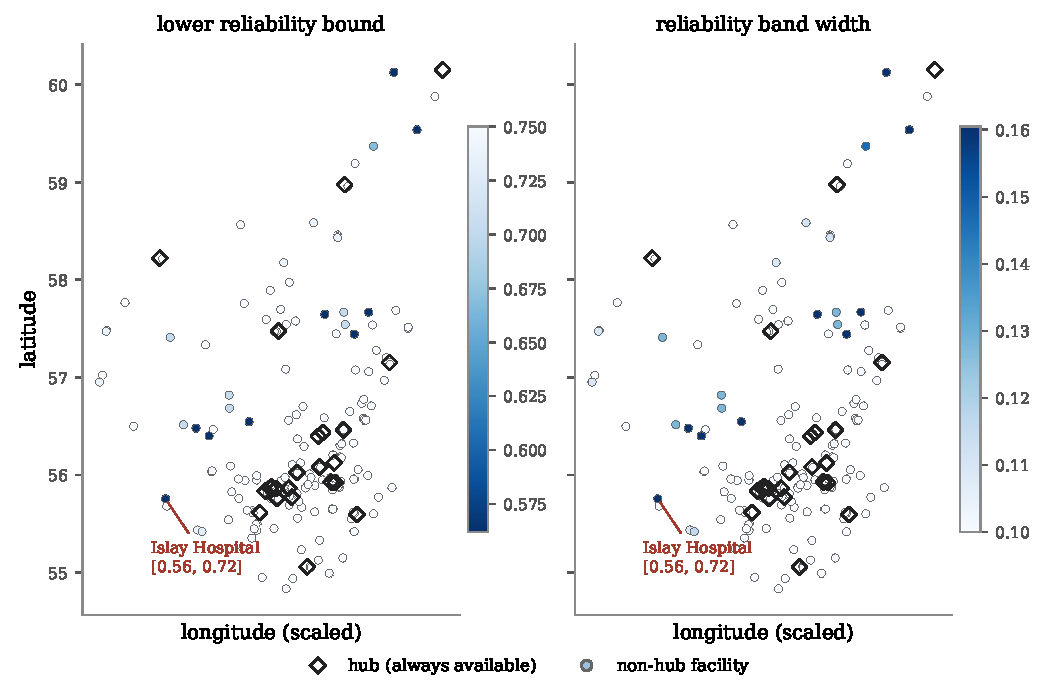
\includegraphics[width=\linewidth]{images/drone_reliability_map.pdf}
\caption{Reliability map of the dense decentralised configuration: each facility coloured by the lower bound of its propagated reachability reliability (left; darker = less certainly reachable) and by the width of its reliability band (right; darker = more uncertainty). Hubs (diamonds) are assumed always available. Uncertainty concentrates at island and far-northern facilities; the worst-served facility, Islay Hospital, is bounded at $[0.56,0.72]$.}
\label{fig:map}
\end{figure}

\subsection{Adversarial Structure}\label{sec:adversarial}

Section~\ref{sec:complexity} used two constructed families, fan-in and mesh, to show where IPA's factorisation helps and where it cannot. This section asks the same question of a real, independently published family, not a hand-built one: the ISCAS85 combinational circuit benchmarks~\cite{brglez_iscas85_1985}, a suite of digital logic circuits represented natively as directed acyclic graphs. Every circuit is assigned the same illustrative, non-degenerate component reliability ($0.9$, uniformly) used throughout this corpus, which is itself a deliberate worst case here: identification excludes a node from a conditioning set only when its reliability is fixed at exactly $0$ or $1$ (Section~\ref{sec:decomp}), so a non-degenerate value everywhere leaves no reconvergent structure excluded from conditioning.

The smallest circuit, \emph{c17} (11 gates), is trivial (conditioning width 1) and was fully validated across all three input types, including a p-box propagation whose cost matched the prediction of Section~\ref{sec:pbox}'s realised-work relationship (predicted $1.3$--$2.3$\,s at 50 discretisation levels; measured $1.41$\,s). The next three circuits tested, \emph{c432} (196 gates), \emph{c499} (243 gates), and \emph{c880} (443 gates), reach conditioning widths of 67, 41, and 50 respectively, an order of magnitude beyond any other network in this corpus, placing exact propagation on these circuits well outside a practical budget; two further circuits, \emph{c1355} and \emph{c1908} (587 and 913 gates), exceed the memory available on a 16\,GB workstation during identification itself.

This is not a boundary specific to IPA. El Fattah and Dechter~\cite{elfattah_diagnosing_1996}, studying the same circuits with classical tree-clustering and cutset conditioning, the general method IPA specialises (Section~\ref{sec:complexity}), independently report clique and cutset sizes for c432 that they describe as ``clearly not feasible'' for any exact structural method, and comparably extreme figures for the larger circuits in the suite. Decision-diagram size is governed by the same structural width, so a well-ordered decision diagram meets the same wall on these circuits; it does not resolve it.

\subsection{Limitations and Future Work}\label{sec:limitations}

\paragraph{Exact point-valued reliability} For point-valued reliability, IPA has no asymptotic advantage over a well-ordered decision diagram: both are exponential in the network's structural width (the conditioning width here, the pathwidth for the diagram), reflecting the \#P-hardness of network reliability, and across the corpus of Section~\ref{sec:comparison} neither dominates. Its distinctive value instead lies in imprecise propagation. Interval results are exact at machine precision, and the speed comparison of Section~\ref{sec:interval} is scoped to one-shot queries. Distributional bounds are sound, but their tightness is structure-dependent, tight for high-reliability or weakly reconvergent systems and conservative for strongly reconvergent systems with broadly uncertain components, and their cost grows with the discretisation level, which confines full distributional propagation to modest networks at present; for larger networks, interval propagation combined with sampling is the practical recourse. The tighter positive-dependence operator is validated empirically but not proven sound in general; every guaranteed claim in this paper uses the proven Fr\'echet operator instead.

\paragraph{Practical range} IPA is exponential in width and intended for the sparse-to-moderate regime, a ceiling shared with every exact method: Section~\ref{sec:adversarial} located it on a real published circuit family, and the applied case study locates it on a real infrastructure network, where a conditioning requirement of 16, reached at sixteen provisioned alternate routes per location, remains practical (tens of seconds), while unrestricted connectivity makes exact diamond identification itself exceed a 16\,GB memory budget before propagation can begin. Imprecise propagation does not relax this boundary: interval and p-box propagation use the same conditioning depth as exact point propagation, and only a change to the network design itself alters the cost. For networks beyond the practical range, a depth-limited hybrid suggests itself: condition exactly to a chosen depth and, beyond it, combine reconvergent contributions without conditioning, which for interval inputs gives a rigorous outer bound (wider, but sound) and for p-box inputs would use the Fr\'echet combination for the unconditioned remainder. This hybrid is proposed, not implemented or evaluated here; the method reported in this paper does not degrade exactness anywhere.

\paragraph{Structural scope} The method addresses directed acyclic dependency structures. The applied case study's networks are directed by the hub-and-spoke supply logic of their source design; general cyclic or bidirectional dependency networks, feedback loops and return flows, are outside the present scope, and their principled treatment, for example by unrolling or by strongly-connected-component condensation, is future work.

The decomposition framework identifies the specific subgraphs responsible for computational intractability, so a natural extension is to apply approximation selectively to deeply nested diamonds while retaining exact computation elsewhere, localising approximation error to the structurally difficult parts of the graph and preserving exactness on the rest.

\section{Conclusions}\label{sec:conclusions}

This paper has presented the Information Propagation Algorithm (IPA), an exact reliability analysis method for directed acyclic process networks with reconvergent dependency structures. The method computes source-to-node reliability by propagating reachability probabilities in topological order, resolves dependent incoming signals by conditioning on separating sets of shared ancestors, and replaces resolved fork--join substructures with statistically equivalent supernodes. IPA is a specialisation of cutset conditioning to source-to-node reachability: its per-instance cost is bounded by $\sum_d 2^{|C_d|}$ over the diamonds resolved, computable before enumeration begins, and an independent-substructure factorisation reduces fan-in conditioning from exponential to linear where independence permits.

Exactness was verified against an independent exact method, a reduced-ordered binary decision diagram with dynamic variable reordering, across 129 random and mutated networks, six topological families, and several structured and real-world networks, with the worst observed disagreement at floating-point precision. The same comparison shows that IPA's cost is governed by the same structural width parameter as the diagram's size, and neither method dominates: for exact point-valued reliability IPA is competitive with, not superior to, a well-ordered decision diagram. Its distinguishing capability is the native propagation of imprecise component reliabilities. Interval-valued inputs yield the exact reliability range at machine precision, faster for one-shot queries than the decision-diagram route to the same interval on every family tested. Probability-box inputs yield guaranteed distributional bounds through a conditioning operator grounded in the Fr\'echet--Hoeffding inequalities, which certify requirement-violation probabilities from a single propagation, a result no point-valued exact method produces analytically.

An applied case study of a medical drone logistics network for Scotland, with every input traced to the source design study and one explicitly flagged extension, illustrates the engineering use of the method: propagated reliability bounds identify the facilities whose delivery reachability is most uncertain under the stated input uncertainty, and a sweep of a real redundancy design parameter locates the practical boundary of exact analysis on the network. Within that boundary, IPA completes full exact propagation in under 25 seconds at a redundancy level where the decision-diagram alternative did not complete within a practical budget. Exact reliability analysis of large acyclic networks is feasible whenever dependency-inducing substructures remain sufficiently localised, and this boundary can be measured and expressed in design terms.

Future work includes a soundness proof for the tighter positive-dependence conditioning operator, the depth-limited hybrid scheme proposed for networks beyond the exact range, extension to multi-state components and explicitly modelled common-cause failures, and a principled treatment of cyclic dependency structures.

\bibliographystyle{elsarticle-num}
\bibliography{references}

\section*{Acknowledgements}
This work was supported by the Nuclear Decommissioning Authority (NDA) in conjunction with the UK National Nuclear Laboratory (UKNNL) through the NDA Bursary Scheme (project number NNL/UA/118).


\section*{Data and Software Availability}

The implementation of the Information Propagation Algorithm (IPA) is released as the open-source Julia package \texttt{InformationPropagationAnalysis.jl}, registered in the Julia General package registry and available at \url{https://github.com/Temi-Tory/InformationPropagationAnalysis.jl}. The benchmark networks, validation scripts, and result artefacts required to reproduce every table and figure in this manuscript are deposited at [Zenodo DOI to be inserted upon minting] under an MIT licence, together with a README mapping each artefact to the manuscript table or figure it supports.

\end{document}

\endinput
%%
%% End of file `elsarticle-template-num.tex'.
    